\documentclass[11pt]{article}
\usepackage{fullpage}
\usepackage{rpmacros}
\RequirePackage[colorlinks=true]{hyperref}
\hypersetup{
  linkcolor=[rgb]{0,0,0.4},
  citecolor=[rgb]{0, 0.4, 0},
  urlcolor=[rgb]{0.6, 0, 0}
}
\usepackage{mathpazo}
\usepackage{bbm}
\usepackage{todonotes}
\usepackage{pgfplots}

\usepackage{lipsum}
\usepackage{setspace}
\usepackage{mdframed}
\usepackage{multicol}
\usepackage{subcaption}
\usepackage{graphicx}
\usepackage{comment}
\usepackage{tikz}
\usetikzlibrary{decorations.pathreplacing,backgrounds}
\usetikzlibrary{plotmarks}

\usepackage[font=footnotesize]{caption}

\usepackage{amsthm}
\usepackage{thmtools,thm-restate}

\numberwithin{equation}{section}
\declaretheoremstyle[bodyfont=\it,qed=\qedsymbol]{noproofstyle} 

\declaretheorem[numberlike=equation]{axiom}

\declaretheorem[numberlike=equation]{observation}
\declaretheorem[numberlike=equation,style=noproofstyle,name=Observation]{observationwp}
\declaretheorem[name=Observation,numbered=no]{observation*}

\declaretheorem[numberlike=equation]{fact}
\declaretheorem[numberlike=equation]{subclaim}
\declaretheorem[numberlike=equation]{problem}

\declaretheorem[numberlike=equation]{theorem}
\declaretheorem[numberlike=equation,style=noproofstyle,name=Theorem]{theoremwp}
\declaretheorem[name=Theorem,numbered=no]{theorem*}

\declaretheorem[numberlike=equation]{lemma}
\declaretheorem[name=Lemma,numbered=no]{lemma*}
\declaretheorem[numberlike=equation,style=noproofstyle,name=Lemma]{lemmawp}

\declaretheorem[numberlike=equation]{corollary}
\declaretheorem[name=Corollary,numbered=no]{corollary*}
\declaretheorem[numberlike=equation,style=noproofstyle,name=Corollary]{corollarywp}

\declaretheorem[numberlike=equation]{proposition}
\declaretheorem[name=Proposition,numbered=no]{proposition*}
\declaretheorem[numberlike=equation,style=noproofstyle,name=Proposition]{propositionwp}

\declaretheorem[numberlike=equation]{claim}
\declaretheorem[name=Claim,numbered=no]{claim*}
\declaretheorem[numberlike=equation,style=noproofstyle,name=Claim]{claimwp}

\declaretheorem[numberlike=equation]{conjecture}
\declaretheorem[name=Conjecture,numbered=no]{conjecture*}

\declaretheorem[numberlike=equation]{question}
\declaretheorem[name=Question,numbered=no]{question*}

\declaretheorem[name=Open Problem]{openproblem}
\declaretheorem[name=Exercise]{exercise}

\declaretheoremstyle[bodyfont=\it,qed=$\lozenge$]{defstyle} 

\declaretheorem[numberlike=equation,style=defstyle]{definition}
\declaretheorem[unnumbered,name=Definition,style=defstyle]{definition*}

\declaretheorem[numberlike=equation,style=defstyle]{example}
\declaretheorem[unnumbered,name=Example,style=defstyle]{example*}

\declaretheorem[numberlike=equation,style=defstyle]{notation}
\declaretheorem[unnumbered,name=Notation=defstyle]{notation*}

\declaretheorem[numberlike=equation,style=defstyle]{construction}
\declaretheorem[unnumbered,name=Construction,style=defstyle]{construction*}

\declaretheorem[numberlike=equation,style=defstyle]{remark}
\declaretheorem[unnumbered,name=Remark,style=defstyle]{remark*}

\renewcommand{\subsectionautorefname}{Section}
\renewcommand{\sectionautorefname}{Section}
\newcommand{\algorithmautorefname}{Algorithm}



%%% Local Variables: 
%%% mode: latex
%%% TeX-master: "main"
%%% End: 

\input{customurlbst/bibmacros}

\usepackage{algorithmicx}
\usepackage{algorithm} % http://ctan.org/pkg/algorithms
\usepackage[noend]{algpseudocode}
\renewcommand{\algorithmicensure}{\textbf{Output:}}
\renewcommand{\algorithmicrequire}{\textbf{Input:}}


\algrenewcommand\algorithmicindent{1.0em}%

\newcommand{\RPnote}[1]{\textcolor{BrickRed}{RP: #1}}
\newcommand{\Mattnote}[1]{\textcolor{OliveGreen}{MWA: #1}}
\newcommand{\BLnote}[1]{\textcolor{Blue}{BLV: #1}}
\newcommand{\Anote}[1]{\textcolor{Plum}{A: #1}}
\newcommand{\MFnote}[1]{\textcolor{DarkOrchid}{MF: #1}}

\newcommand*\samethanks[1][\value{footnote}]{\footnotemark[#1]}
\newcommand\sse{\subseteq}
\newcommand\Sym[1]{\ensuremath{\mathrm{Sym}_{#1}}}
\newcommand\condset[2]{\set{#1 \;|\; #2}}
\renewcommand\NP{\ensuremath{\mathsf{NP}}}
\newcommand\coNP{\ensuremath{\mathsf{coNP}}}

%\onehalfspacing
\date{}

\title{Matrix Multiplication: \\Verifying Strong Uniquely Solvable Puzzles
{\IfFileExists{./sha.tex}{\\\small SHA: \input{sha}}{}}}
\author{
Matthew Anderson\thanks{Department of Computer Science, Union College, Schenectady, New York, USA, E-mails: \texttt{andersm2@union.edu, jiz@union.edu, xua@union.edu}}%
\and%
Zongliang Ji\samethanks[1]
\and%
Anthony Yang Xu\samethanks[1]
}
\begin{document}
\maketitle

\begin{abstract}
Cohn and Umans proposed a framework for developing fast matrix
multiplication algorithms based on the embedding computation in
certain groups \cite{cu03}.  Subsequent work with Kleinberg and
Szegedy connected this to the search for combinatorial objects called
strong uniquely solvable puzzles (SUSP) \cite{cksu05}.  We begin a
systematic computer-aided search for these objects.  We develop and
implement algorithms and heuristics to verify that puzzles are SUSP
and to search for large ones.  We produce tight bounds on the maximum
size of puzzles for width $k < 6$, and construct puzzles of small
width that are larger than previous work.  Although our work only
deals with puzzles of small-constant width and does not produce a new
faster algorithm, it gives evidence that there exist families of SUSP
that imply matrix multiplication algorithms that are more efficient
than those currently known.
\end{abstract}

\thispagestyle{empty}
\newpage
\pagenumbering{arabic}


\section{Introduction}
\label{sec:intro}

% Context

An optimal algorithm for matrix multiplication remains elusive
despite substantial effort.  Here we focus on the square variant of the
matrix multiplication problem, i.e., given two $n$-by-$n$ matrices
$A$ and $B$ over a field $\F$, the goal is to compute the matrix
product $C = A \times B$.  The outstanding open question is: How many field
operations are required to compute $C$?  The long thought-optimal na\"{i}ve algorithm,
based on the definition of matrix product is $O(n^3)$ time.
The groundbreaking work of Strassen showed that it can
be done in time $O(n^{2.808})$ \cite{str69} using a
divide-and-conquer approach.  A long sequence of work concluding with
Coppersmith and Winograd's algorithm (CW) reduced the running time
to $O(2^{2.376})$ \cite{pan78,sch81,str86,cw90}. Recent
computer-aided refinements of CW by others reduced the
exponent to $\omega \le 2.3728639$ \cite{ds13,wil12,le14}.

% Motivation

Cohn and Umans \cite{cu03} introduced a framework for developing
faster algorithms for matrix multiplication by reducing this 
to a search for groups with subsets that satisfy an algebraic
property called the \emph{triple-product property} that allows matrix
multiplication to embed in the group algebra.  Subsequent work
\cite{cksu05} elaborated on this idea and developed the notion of
combinatorial objects called \emph{strong uniquely solvable puzzles}
(SUSP) whose existence would also imply faster matrix multiplication
algorithms.

A \emph{width}-$k$ puzzle $P$ is a subset of $\set{0,1,2}^k$,
and the cardinality of $P$ is the puzzle's \emph{size}.  Each element
of $P$ is called a \emph{row} of $P$, and each row consists of three
\emph{subrows} that are elements of $\set{0,*}^k$, $\set{1,*}^k$,
$\set{2,*}^k$ respectively.  Informally, a puzzle $P$ is a
\emph{uniquely solvable puzzle} (USP) if there is no way to permute
the subrows of $P$ without overlap to form a distinct puzzle $P'$.  A
uniquely solvable puzzle is \emph{strong} if a tighter condition for
non-overlapping is applied. For a fixed
width $k$, the larger the size of a strong USP $P$, the faster matrix
multiplication algorithm it implies \cite{cksu05}.  In fact Cohn et
al.~show that there exist an infinite family of SUSP that achieves
$\omega < 2.48$.

% Approach

We follow Cohn et al.'s program by: (i) developing \textbf{verification}
algorithms to determine whether a puzzle is a SUSP, (ii) developing
\textbf{search} algorithms to find large SUSP, and (iii) creating and
runnning practical \textbf{implementations} of these algorithms.  The
algorithms we develop are not efficient as they run in exponential
time in the natural parameters.  However, the goal is to find a
sufficiently large SUSP that imply a faster matrix
multiplication algorithm, and the resulting algorithm's running time
is independent of the running time of our algorithms.  The
inefficiency of our algorithms limit the search space that
we can practically examine.

% Results

In addition to creating algorithms, we have experimental results that
bound the size of the largest SUSP for small-width puzzles.  For
small-constant width, $k \le 12$, we beat the largest sizes of
\cite[Proposition 3.8]{cksu05}.  Our lower bounds on max size are
witnessed by SUSP we found via search.  For $k \le 5$ we give tight
upper bounds determined by exhaustively searching all puzzles.
Although our current experimental results do not beat \cite{cksu05}
for unbounded $k$, they may give evidence that there exist families of
SUSP that imply matrix multiplication algorithms that are more
efficient than those currently known.

There are a number of negative results in known.  Na\"{i}vely, the
dimensions of the output matrix $C$ imply that the problem requires at
least $\Omega(n^2)$ time.  Slightly better lower bounds are known in
general and also for specialized models of computation, c.f., e.g.,
\cite{shp03,kam05}.  There are also lower bounds known for a variety
of algorithmic approaches to matrix multiplication.  Ambainis et
al.~showed that the laser method cannot alone achieve an algorithm
with $\omega \le 2.3078$ running time \cite{afl15}.  A recent
breakthrough arithmetic progressions in cap sets \cite{clp17} combined
with a conditional result on the Erd\"{o}s-Szemeredi sunflower
conjecture \cite{asu13} imply that Cohn et al.'s strong uniquely
solvable puzzle approach cannot achieve the $\omega = 2 + \epsilon$
for some $\epsilon > 0$ \cite{bccgu16}.  Subsequent work has
generalized this barrier \cite{avw18a,avw18b} to a larger class of
algorithmic techniques.  Despite this, we are unaware of a concrete
lower bound on $\epsilon$ implied by these negative results.  There
remains a substantial gap in our understanding between what has been
acheived by the positive refinements of LeGall, Williams, and
Stothers, and the impossibility of showing $\omega = 2$ using the
strong USP approach.

\smallskip
% Organization
%\paragraph{Organization}
\noindent\textbf{Organization} \autoref{sec:prelim} begins with the formal definition of strong USP.
In \autoref{sec:verify} we discuss our algorithms for verifying that a
puzzle is a strong USP.  In \autoref{sec:heuristic} we describe fast,
but incomplete, heuristics for verifying strong USP.
\autoref{sec:search} explains our search algorithms.
\autoref{sec:results} discuss our experimental results.


\section{Preliminaries}
\label{sec:prelim}

\newcommand\ordset[1]{\ensuremath{[#1]}}

We use $\ordset{n}$ to denote the set $\set{0,1,2,\ldots, n-1}$.  For
a set $Q$, $\Sym{Q}$ denotes the symmetric group on the elements of
$Q$.
%We use $1$ to denote the identity permutation in
%$\Sym{Q}$.
Cohn et al.~introduced the idea of a \emph{puzzle}.
\begin{definition}[Puzzle]
  For $s, k \in \Natural$, an $(s,k)$-\emph{puzzle} is a
  subset $P \sse \ordset{3}^k$ with $|P| = s$.
\end{definition}
\noindent We say that an $(s,k)$-puzzle has $s$ rows and $k$ columns.  The
columns are inherent ordered and indexed by $\ordset{k}$.  The rows
are not inherently ordered, however, it is often convienent to assume
that the rows are arbitrarily ordered and indexed by $\ordset{s}$.

\cite{cksu05} also establish a particular combinatorial property of
such puzzles that can derive group algebras that matrix multiplication can be
embedded into.  Such puzzles are called \emph{strong uniquely
solvable puzzles}.

%% However, to give some intuition we first explain a
%% simpler version of the property called \emph{uniquely solvable
%%   puzzles}.

%% \begin{definition}[Uniquely Solvable Puzzle (USP)]

%%   ~\\An $(s,k)$-puzzle $P$ is \emph{uniquely solvable} if
%%   $\forall \pi_0, \pi_1, \pi_2 \in \Sym{P}:$
%%   \begin{enumerate}
%%   \item either $\pi_0 = \pi_1 = \pi_2$, or
%%   \item $\exists r \in P, \exists i \in \ordset{k}$ such that at least two
%%     of the following hold:
%%     \begin{enumerate}
%%     \item $(\pi_0(r))_i = 0$,
%%     \item $(\pi_1(r))_i = 1$,
%%     \item $(\pi_2(r))_i = 2$.
%%     \end{enumerate}
%%   \end{enumerate}
%% \end{definition}

%% Informally, a puzzle is \textbf{not} uniquely solvable if each row of
%% the puzzle can be broken into zeroes, ones, and twos pieces and then
%% the rows can be reassembled in a different way so that each new row is
%% a combination of a zeroes, a ones, and twos piece where there is
%% exactly one element of $\ordset{3}$ for each column.  Observe that
%% uniquely solvable puzzles can have at most $2^k$ rows because each
%% zeroes piece, ones piece, and two piece must be unique, as otherwise
%% the duplicate pieces can be swapped making the puzzle not uniquely
%% solvable.  The definition of \emph{strong} uniquely solvable puzzle is
%% below, it is nearly the same except that it requires that there be a
%% collision on a column between exactly two pieces, not two or more
%% pieces like in the original definition.

\begin{definition}[Strong Uniquely Solvable Puzzle]
  \label{def:strong-USP}
  An $(s,k)$-puzzle $P$ is \emph{strong uniquely solvable} if for all
  $\pi_0, \pi_1, \pi_2 \in \Sym{P}$: Either (i) $\pi_0 = \pi_1 = \pi_2$,
  or (ii) there exists $r \in P$ and $i \in \ordset{k}$ such that exactly
  two of the following hold: $(\pi_0(r))_i = 0$, $(\pi_1(r))_i = 1$,
  $(\pi_2(r))_i = 2$.
\end{definition}

\noindent Observe that the properties of uniquely solvable and strong uniquely
solvable are invariant to the ordering of the rows or columns of a
puzzle.  This fact is used implicitly.
%Note that if a puzzle $P$ is a
%SUSP then it is also a USP.
%% Further note that these properties are
%% invariant to maps between puzzles induced by permutations from
%% \Sym{\ordset{3}} on the puzzle cell elements.

Cohn et al.~show the following connection between the existence of
strong uniquely solvable puzzles and upper bounds on the exponent of
matrix multiplication $\omega$.
\begin{lemma}[{\cite[Corollary 3.6]{cksu05}}]
  \label{lem:omega}
  If there is a strong uniquely solvable $(s,k)$-puzzle,
  $$\omega \le \min_{m \ge 3, m \in \Natural} \frac{3 \log
    m}{\log(m-1)} - \frac{3 \log s!}{sk \log(m-1)}.$$
\end{lemma}
%% \noindent In the same article, the authors also demonstrate the
%% existence of an infinite family of strong uniquely solvable puzzles,
%% for width $k$ divisible by three, that achieves a non-trivial bound on
%% $\omega$.
%% \begin{lemma}[{\cite[Proposition 3.8]{cksu05}}]
%%   There is an infinite family of strong uniquely solvable puzzles that
%%   achieves $\omega < 2.48$.
%% \end{lemma}
%% \noindent Finally, they conjecture that strong uniquely solvable
%% puzzles provide a root to achieving quadratic time matrix
%% multiplication.
%% \begin{conjecture}[{\cite{cksu05}}]
%%   There exists a family of strong uniquely solvable puzzles that
%%   implies $\omega = 2$.
%% \end{conjecture}
%% \noindent Unfortunately, as mentioned in the introduction, this
%% conjecture was recently shown to be false.
%% \begin{lemma}[\cite{bccgu16}]
%%   Strong uniquely solvable puzzles cannot show $\omega < 2 +
%%   \epsilon$, for some $\epsilon > 0$.
%% \end{lemma}
%% \noindent That said, there remains hope that the uniquely solvable
%% puzzle approach could beat the refinements of Coppersmith-Winograd
%% even if it cannot reach $\omega = 2$.

%% \noindent This result is a consequence of a recent breakthrough
%% arithmetic progressions in cap sets \cite{e16,clp16} combined with a
%% conditional result on the Erd\"{o}s-Szemeredi sunflower conjecture
%% \cite{asu13}.  The results of \cite{bccgu16} do imply that Cohn and
%% Umans' strong uniquely solvable puzzle approach cannot achieve the
%% ideal $\omega = 2$.  However, we are unaware of a concrete lower bound
%% on $\epsilon$ implies by this result.  This means there is a still a
%% substantial gap in our understanding between what has been acheived by
%% the refinements of LeGall, Williams, and Stothers, and the
%% impossibility of showing $\omega = 2$ using the Cohn and Umans'
%% approach.



\section{Verifying Strong USPs}
\label{sec:verify}

The core focus of this article is the verification of strong USP:
Given an $(s,k)$-puzzle $P$, output YES iff $P$ is a strong USP.  In
this section we discuss the design of algorithms to solve this problem
as a function of the natural parameters $s$ and $k$.
%% As the goal of this work is to actually 
%% to use computers to locate large strong USPs,
Along the way we also discuss some aspects of our practical
implementation that informed or constrained our designs.  All the
exact algorithms we develop in this section have exponential running
time.  However, asymptotic worst-case running time is not the metric
we are truly interested in.  Rather we are interested in the practical
performance of our algorithms and their capability for locating new
large strong USP.  The algorithm that we ultimately develop is a
hybrid of a number of simpler algorithms and heuristics.

%% The reason
%% for this is that the algorithms with better asymptotic and practical
%% performance at larger input lengths have large overhead at small input
%% lengths.

%% XXX - commented out below, but should this be somewhere else? It doesn't
%% feel like it should be here.
%%
%% The parameters $s$ and $k$ they are not fully independent.  First,
%% $s \le 3^k$ because the maximum number of rows in a puzzle of width
%% $k$ is $|[3]^k| = 3^k$.  Second, we can eliminate the dependence on
%% $k$ entirely by transforming an $(s,k)$-puzzle into a 3D matching
%% instance on the vertex set $[s]^3$.  However, this transformation is
%% not free because the instance size is now a function of the cube of
%% $s$ rather than linear in $s$.

\subsection{Brute Force}

The obvious algorithm for verification comes directly from the
definition of strong USP.  Informally, we consider all ways of
permuting the ones and twos pieces relative to the zeroes pieces and
check whether the non-overlapping condition of
\autoref{def:strong-USP} is met.  A formal description of the
algorithm is found \autoref{alg:brute-force}.


\begin{algorithm}[t]
  \caption{: Brute Force}
  \label{alg:brute-force}
\begin{algorithmic}[1]
  \Require{An $(s,k)$-puzzle $P$.}
  \Ensure{YES, if $P$ is a strong USP and NO otherwise.}
  \Function{VerifyBruteForce}{$P$}
  \For{$\pi_1 \in \Sym{P}$}
    \For{$\pi_2 \in \Sym{P}$}
      \If{$\pi_1 \neq 1 \vee \pi_2 \neq 1$}
        \State{$found = false.$}
        \For{$r \in P$}
          \For{$i \in [k]$}
            \If{$\delta_{r_i, 0} + \delta_{(\pi_1(r))_i, 1} + \delta_{(\pi_2(r))_i, 2} = 2$} $found = true$. \EndIf
          \EndFor
        \EndFor
        \If{\textbf{not} $found$} \Return{NO.} \EndIf
      \EndIf
    \EndFor
  \EndFor
  \State{\Return{YES}.}
  \EndFunction
\end{algorithmic}
\end{algorithm}

The $1$ in Line 4 of \autoref{alg:brute-force} denotes the
identity in $\Sym{P}$, and $\delta_{a,b}$ is the Kronecker delta
function which is $1$ if $a = b$ and $0$ otherwise.  Observe that
\autoref{alg:brute-force} does not refer to $\pi_0$ of
\autoref{def:strong-USP}.  This is because the strong USP property is
invariant to permutations of the rows and so $\pi_0$ can be thought of
as an arbitrary phase.  Hence, fix $\pi_0 = 1$ to simplify the
algorithm.  Seeing that $|\Sym{P}| = s!$, we conclude that the algorithm
runs in time $O((s!)^2 \cdot s \cdot k \cdot \poly(s))$ where the last
factor accounts for the time to perform operations on permutations of
$s$ elements.  The dominant term in the running time is the
contribution from iterating over pairs of permutations.
%, though this
%term was made a factor $s!$ smaller by not iterating over $\pi_0$.
Finally, notice that if $P$ is a strong USP, then the algorithm runs
in time $\Theta((s!)^2 \cdot k \cdot \poly(s))$, and that if $P$ is
not a strong USP the algorithm terminates early.  The algorithm's
poor performance made it unusable in our
implementation, however, it's simplicity and direct connection to the
definition made its implementation a valuable sanity check against
later more elaborate algorithms (and it served as effective onboarding to
the undergraduate students collaborating on this project).

Although \autoref{alg:brute-force} performs poorly, examining the
structure of a seemingly trivial optimization leads to substantially
more effective algorithms. Consider the following function on triples
of rows $a, b, c$: $f(a,b,c) = \vee_{i \in [k]} (\delta_{a_i,0} +
\delta_{b_i,1} + \delta_{c_i,2} = 2).$ We can replace the innermost
loop in Lines 7 \& 8 of \autoref{alg:brute-force} with the statement
$found = found \vee f(r, \pi_1(r), \pi_2(r))$.  Observe that $f$
neither depends on $P$, $r$, nor the permutations, and that
\autoref{alg:brute-force} no longer depends on directly on $k$.  To
slightly speed up \autoref{alg:brute-force} we can precompute and
cache $f$ before the algorithm starts and then look up values as the
algorithm runs.  We precompute $f$ specialized to the rows in the
puzzle $P$, and call it $f_P$.

%% There are two obvious options to consider we can
%% either precompute $f$ specialized to the rows in the puzzle $P$, or we
%% can precompute $f$ for all possible rows.
%% In former case the time to
%% precompute $f$ is $\Theta(s^3 \cdot k)$ and in the later case
%% $\Theta(3^{3k} \cdot k)$.  The storage requirements are $\Theta(s^3)$
%% and $\Theta(3^{3k})$ bits respectively.  The former is problematic for
%% large $s$ and later problematic even for small $k$.  Moreover the
%% combined running time for the two options with a single call to verify
%% a puzzle is $\Theta(s^3 \cdot k + (s!)^2 \cdot \poly(s))$ and
%% $\Theta(3^{3k} \cdot k + (s!)^2 \cdot \poly(s))$.  In the former case
%% there is an asymptotic improvement, but in the later case, the saving
%% of a factor of $k$ is easily offset by the additional $3^{3k}$ term.
%% For this reason we rule out the later option and chose to represent
%% the function $f$ specialized to $f_P$ for a given puzzle $P$.


\subsection{Verification to 3D Matching}
\label{sec:3DM}

For verification it turns out to be more useful to work with $f_P$
than with $P$.  It is convienent to think of $f_P$ from several
perspectives: (i) as a function $f_P : P \times P \times P \rightarrow
\set{0, 1}$,
%(ii) as an order-three tensor $f_p \in \set{0,1}^{P \times P \times P}$,
and (ii) as the complement of the
characteristic function of relations of a tripartite
hypergraph $H_P = \langle P \sqcup P \sqcup P, \bar{f_p}\rangle$ where
the vertex set is the disjoint union of three copies of $P$.  The latter of these, $H_P$, is the most useful.

Let $G = \langle P \sqcup P \sqcup P, E \sse P^3\rangle$ be a
tripartite 3-hypergraph.  We say $G$ has a \emph{3D matching} iff
there exists a subset $M \sse E$ with $|M| = |P|$ and for all distinct
hyperedges $e_1, e_2 \in M$, $e_1$ and $e_2$ are \emph{vertex
  disjoint}, i.e., $(e_1)_i \neq (e_2)_i$ for all $i \in [3]$.  A 3D matching is \emph{non-trivial} if it is not the matching
$\condset{(r,r,r)}{r \in P}$.  The existence of 3D matchings in $H_P$
is directly tied to whether $P$ is a strong USP.

\begin{lemma}
  \label{lem:verify-to-3dm}
  An $(s,k)$-puzzle $P$ is a strong USP iff $H_P$ has no non-trivial 3D
  matching.
\end{lemma}

\begin{proof}
  We first argue the reverse.  Suppose that $H_p$ has a
  non-trivial 3D matching $M$.  We show that $P$ is not a strong USP by
  using $M$ to construct $\pi_0, \pi_1, \pi_2 \in \Sym{P}$ that
  witness this.  Let $\pi_0$ be the identity permutation.  For each $r
  \in P$, define $\pi_1(r) = q$ where $(r,q,*) \in M$.  Note that $q$
  is well defined and unique because $M$ is 3D matching and so has
  vertex disjoint edges.  Similarly define $\pi_2(r) = q$ where
  $(r,*,q) \in M$.  Observe that by construction $M =
  \condset{(\pi_0(r),\pi_1(r),\pi_2(r))}{r \in P}$.  Since $M$ is a
  matching of $H_P$, $M \sse \bar{f_P}$.  Because $M$ is a non-trival
  matching at least one edge in $(a,b,c) \in M$ is has either $a \neq
  b$, $a \neq c$, or $b \neq c$.  This implies, respectively, that as
  constructed $\pi_0 \neq \pi_1$, $\pi_0 \neq \pi_2$, or $\pi_1 \neq
  \pi_2$.  In each case we have determined that $\pi_0$, $\pi_1$, and
  $\pi_2$ are not all identical.  Thus we determined permutations such
  that for all $r \in P$, $f(\pi_0(r), \pi_1(r), \pi_2(r)) = 0$.  This
  violates Condition (ii) of \autoref{def:strong-USP}, hence $P$ is not a
  strong USP.

  The forward direction is symmetric.  Suppose
  that $P$ is not a strong USP. We show that $H_P$ has a 3D matching.
  For $P$ not to be a strong USP there must exist $\pi_0, \pi_1, \pi_2
  \in \Sym{P}$ not all identical such that Condition (ii) of
  \autoref{def:strong-USP} fails.  Define $e(r) =
  (\pi_0(r),\pi_1(r),\pi_2(r))$ and $M = \condset{e(r)}{r \in P}$.
  Since Condition (ii) fails, we have that $f_P(e(r)) = false$ for all $r
  \in P$.  This means that for all $r \in P$, $e(r) \in \bar{f_P}$ and
  hence $M \sse \bar{f_P}$.  Since $\pi_0$ is a permutation, $|M| =
  |P|$.  Observe that $M$ is non-trivial because not all 
  the permutations are identical and there must be some $r \in P$ with
  $e(r)$ having non-identical coordinates.  Thus $M$ is a non-trivial
  3D matching.
\end{proof}

Note that although 3D matching is an \NP-complete problem \cite{gj79},
\autoref{lem:verify-to-3dm} does not immediately imply that
verification of strong USP is \coNP-complete because $H_P$ is not an
arbitrary hypergraph.  (That verification is in \coNP{} is immediate
from \autoref{def:strong-USP}.)
%Indeed, it seems difficult to define
%a puzzle $P$ that allows hyperedges in $H_P$ to be included
%independently.
It remains open whether verification is
\coNP-complete.
%, but our experimental data suggests
%that it may not to be the case.
\autoref{lem:verify-to-3dm} implies that to verify $P$ is a strong USP
it suffices to determine whether $H_P$ has a 3D matching.  In the
subsequent sections we examine algorithms for the later problem.  We
can, in retrospect, view \autoref{alg:brute-force} as algorithm for solving 3D
matching.
%% Since we believe that verification is not \coNP-complete we
%% use properties of strong USP and puzzles to provide additional
%% structure that algorithms can take advantage of.

%XXX - Discuss simplifyTDM.  Nope...

\subsection{Bidirectional Search}

The realization that verification of strong USP is a variant of 3D
matching quickly led to a linear exponential time algorithm that was
more practical.  The reduction allows us to replace the permutations
from $\Sym{P}$ with subsets of $P$ and effectively reduce the cost of
the outer loops of \autoref{alg:brute-force} from $s! =
\Theta(2^{s\log s})$ to $2^s$.  This results in a dynamic programming
algorithm for strong USP verification that takes time $O(2^{2s} \poly(s) +
\poly(s,k))$.  For space, we defer the details of the algorithm to
\autoref{app:bi}.

\subsection{3DM to 3SAT}
\label{subsec:sat}

By \autoref{lem:verify-to-3dm}, one can determine whether a puzzle $P$
is a strong USP by contructing a graph $H_P$ from $P$ and deciding
whether it has a non-trivial 3D matching.  It well-known that 3D
matching is \NP{}-complete, c.f., e.g., \cite{gj79}, and that it can be
efficiently reduced to other \NP{}-complete problems. Here we reduce
our 3D matching problem to the CNF satisfability (SAT) problem and
then use a state-of-the-art SAT solver (MapleCOMPSPS \cite{lgpc16}) to
answer the reduced problem. To perform the reduction, we convert the
graph $H_P$ that is obtained from the puzzle $P$ into a conjunctive
normal form (CNF) formula, $\Psi_P$, a depth-2 formula that is the AND
of ORs of Boolean literals.  We input the CNF formula $\Psi_P$ into a
SAT solver to determine whether the formula is satisfiable.  We
construct $\Psi_P$ so that \autoref{lem:verify-to-3dm} implies that
$\Psi_P$ is satisfiable iff $H_P$ has a non-trivial \emph{3D
  matching}.

Let $H_P = \langle V, E \rangle$ be the 3D matching instance
associated with the puzzle $P$.  Our goal is to construct a
non-trivial 3D matching $M$ that is a subset of the edges of $E$ and
is vertex disjoint.
%% We use $M_{u,v,w}$ to denote a variable with
%% values in $\set{0,1}$ that indicates whether the edge $(u,v,w) \in
%% P^3$ is present in the matching.
%% We describe the clauses of the CNF formula $\Phi_P$ whose
%% satisfiability captures the existence of a 3D matching in $H_P$.
%% First, we have clauses that prevents non-edges from being included:
%% \begin{equation}
%%   \Phi_P^{\text{non-edge}} = \bigwedge_{(u,v,w) \in \overline{E}} \neg M_{u,v,w}.
%% \end{equation}
%% Note that, alternatively, we could just eliminate these variables by
%% replacing them by constant false in the subsequent formula. Second, we
%% add clauses that require that every vertex in $H_P$ is matched with
%% some hyperedge:
%% \begin{equation}
%%   \Phi_P^{\ge 1} = 
%%   \left(\bigwedge_{u \in P}\vee_{v,w \in P} ~M_{u,v,w}\right)
%%   \wedge \left(\bigwedge_{v \in P}\vee_{u,w \in P} ~M_{u,v,w}\right)
%%   \wedge \left(\bigwedge_{w \in P}\vee_{u,v \in P} ~M_{u,v,w}\right).
%% \end{equation}
%% Note that three types of clauses above account for the three disjoint
%% copies of $P$ in the vertices of $H_P$.  Third, we require that each
%% vertex can only be matched one a single hyperedge and so have clauses
%% that exclude matching hyperedges that overlap non-trivially (on one or
%% two coordinates):
%% \begin{equation}
%%   \Phi_P^{\le 1} = \bigwedge_{(u,v,w), (u',v',w') \in P^3} (u = u'
%%   \vee v = v' \vee w = w') \wedge (u,v,w \neq u',v',w') \Rightarrow
%%   \neg M_{u,v,w} \vee \neg M_{u',v',w'}.
%% \end{equation}
%% Fourth, we exclude the trivial 3D matching by requiring that at least
%% one of diagonal hyperedges not be used:
%% \begin{equation}
%%   \Phi_P^{\text{non-trivial}} = \bigvee_{u \in P} \neg M_{u,u,u}.
%% \end{equation}
%% Finally, we AND these into the overall formula:
%% \begin{equation}
%%   \Phi_P = \Phi_P^{\text{non-edge}} \wedge \Phi_P^{\le 1} \wedge
%%   \Phi_P^{\ge 1} \wedge \Phi_P^{\text{non-trivial}}.
%% \end{equation}
%% The size of the CNF formula $\Phi_P$ dominated by the size of
%% $\Phi_P^{\le 1}$ which is $\Theta(s^5)$ size.  This is relatively
%% large compared to the $\Theta(s^3)$ size required to represent the
%% hyperedges of the 3DM instance.
%% To avoid the polynomial growth in instance size we decided to use a
%% more concise matching representation.

A na\"{i}ve reduction would be to have variables $M_{u,v,w}$ indicating inclusion of each
hyperedge $(u,v,w) \in P^3$ in the matching. This results in a formula with
$s^3$ variables and size $\Theta(s^5)$.
For greater concision we uses sets
of variables to indicate which vertices in the second and third part
are matched with each vertex in the first part.  In particular we have
Boolean variables $M_{u,v}^1$ and $M_{u,w}^2$ for all $u, v, w \in P$,
and these variable map to assignments in the original scheme in the
following way: $M_{u,v}^1 \wedge M_{u,w}^2 \Leftrightarrow M_{u,v,w}$.

We can rewrite our CNF formula for 3D matching using these
variables.  First, we have clauses that prevents non-edges from
being in the matching:
%\begin{equation}
  $\Psi_P^{\text{non-edge}} = \bigwedge_{(u,v,w) \in \overline{E}}
  (\neg M_{u,v}^1 \vee \neg M_{u,w}^2).$
%\end{equation}
Next, we add clauses require that every vertex in $H_P$ is matched with some
hyperedge:
\begin{equation}
  \Psi_P^{\ge 1} =
  \left(\bigwedge_{u \in P} (\vee_{v\in P} ~M_{u,v}^1) \wedge (\vee_{w \in P} ~M_{u,w}^2)\right)
  \wedge \left(\bigwedge_{v \in P} (\vee_{u \in P} ~M_{u,v}^1)\right)
  \wedge \left(\bigwedge_{w \in P} (\vee_{u \in P} ~M_{u,w}^2)\right).
\end{equation}
Note that these clauses are no longer symmetric because the first part
of $H_P$ is considered in both sets of variables.

Third, we require that each vertex can only be matched one a single
hyperedge and so have clauses that exclude matching hyperedges that
overlap non-trivially (on one or two coordinates).
\begin{equation}
  \Psi_P^{\le 1} = \bigwedge_{i \in \set{1,2}} \bigwedge_{(u,v),
    (u',v') \in P^2} (u = u' \vee v = v') \wedge (u,v \neq u',v')
  \Rightarrow \neg M_{u,v}^i \vee \neg M_{u',v'}^i.
\end{equation}
Observe that $\Psi_P^{\le 1}$ has size $\Theta(s^3)$ compared to the
size of the original $\Phi_P^{\le 1}$ that had size $\Theta(s^5)$.
Fourth, we exclude the trivial 3D matching by requiring that at least
one of diagonal hyperedges not be used:
%\begin{equation}
  $\Psi_P^{\text{non-trivial}} = \bigvee_{u \in P} \neg M_{u,u}^1 \vee
  \neg M_{u,u}^2.$
%\end{equation}
Finally, we AND these into the overall formula:
%\begin{equation}
  $\Psi_P = \Psi_P^{\text{non-edge}} \wedge \Psi_P^{\le 1} \wedge
  \Psi_P^{\ge 1} \wedge \Psi_P^{\text{non-trivial}}.$
%\end{equation}
The size of the CNF formula $\Psi_P$ is $\Theta(s^3)$, has $2s^2$
variables, and is a factor of $s^2$ smaller than the na\"{i}ve
approach.  Thus we reduce 3D matching to satisfiability by converting the
instance $H_P$ into the CNF formula $\Psi_P$.  At this point the
reduction is straightforward, but is included for completeness in
\autoref{app:sat}.

As mentioned before, to solve the satisfiability problem %to implement Line 4 of \autoref{alg:sat}
in
practice we used the solver MapleCOMPSPS, from the 2016
international SAT competition \cite{bhj17,lgpc16}.  This solver is
conflict driven and uses a learning rate branching heuristic to decide
which variables are likely to lead to a conflict.  The solver provides
no polynomial-time worse run time guarantees, but has had
demonstratable success in practice.

\subsection{3DM to IP}

Another way to utilize the connection between verification of strong
USP and 3D matching is to further reduce 3D matching to integer
programming, another well-known \NP{}-complete optimization problem.
Let $H_P = \langle V, E \rangle$ be the 3D matching instance
associated with the puzzle $P$.  Our goal is to construct a
non-trivial 3D matching $M$ that is a subset of the edges of $E$ and
is vertex disjoint.  We use $M_{u,v,w}$ to denote a variable with
values in $\set{0,1}$ that indicates whether the edge $(u,v,w) \in
P^3$ is present in the matching.

To ensure that $M$ is a subset of $E$ we require the following edge constraints
\begin{equation}
  \forall u,v,w \in P,~~M_{u,v,w} \le \begin{cases} 0, (u,v,w) \not\in
    E, and \\ 1, (u,v,w) \in E.\end{cases} \label{eqn:cons1}
\end{equation} We also require that each vertex in
each of the three parts of the graph is incident to exactly one edge
in $M$.  This is captured by the following vertex constraints:
\begin{equation}
  \label{eqn:cons2}
\begin{aligned}
&\forall w \in P,~~\sum_{u,v \in P} M_{u,v,w} = 1,\\
&\forall v \in P,~~\sum_{u,w \in P} M_{u,v,w} = 1,\text{and} \\
&\forall u \in P,~~\sum_{v,w \in P} M_{u,v,w} = 1.
\end{aligned}
\end{equation}
Lastly, since we need that the 3D matching be non-trivial we
add the constraint:
%\begin{equation}
%\label{eqn:cons3}
  $\sum_{u \in P} M_{u,u,u} < |P|.$
%\end{equation}


%% With these constraints in mind, \autoref{alg:mip} describes the
%% overall reduction.

%% By this theory, \autoref{alg:mip} would first transfers input puzzle
%% $P$ into a tripartite hypergraph $H_p$ and creates an empty mixed
%% integer programming model. For every hyperedge $e= \notin H_p$, a
%% constrain $f(e) = 0$ is added into the model as it can not be selected
%% into subset $M$. Afterward the algorithm would also add the
%% restrictions listed in the paragraph above (I am not sure if I should
%% list all the constrains again?). Finally, the model is put through a
%% integer programming solver. If the model has a solution, $H_p$ has a
%% non-trivial 3D matching and by \autoref{lem:verify-to-3dm} $P$ is not a
%% USP. Otherwise if the model is infeasible, $H_p$ does not have a
%% non-trivial thus $P$ is a USP.

To check whether $P$ is a strong USP we need to determine that the
above integer program is not feasible,
%The heavy lifting in \autoref{alg:mip} occurs in Line 5 where the
%integer program is checked for feasibility,
i.e., that there is no
assignment to the variables $M$ that satisfy all the constraints.  In
practice we hand off this computation to the third-party mixed-integer
programming solver Gurobi \cite{gurobi}.  It should be noted that
Gurobi is a commerical, closed-source solver, so we cannot necessarily
verify its assertion that the integer program $Q$ is infeasible.  On
the otherhand, when it determines that the integer program $Q$ is
feasible, we can verify that the solution it produced is a witness of
feasibility.  Further, Gurobi provides no asymptotic performance
guarantees, must less polynomial ones.  We do note that reduction from
3D matching to IP is polynomial time as $H_P$ can be efficiently
constructed from $P$ and there are $s^3 + 3s^3 + 1 = O(s^3)$
constraints and $s^3$ variables in the integer program $Q$.
 
\label{subsec:mip}




\subsection{Heuristics}
\label{sec:heuristic}

Despite our efforts devise an exact algorithm for verifying strong
USPs, the performance of the final algorithm was not practical.  To
speed the algorithm up we considered a number of verification
heuristics that were fast to evaluate, but did not alway produce a
definitive answer.  The heuristics output YES, NO, or MAYBE to whether
a given puzzle $P$ was a strong USP.  We consider only Las Vegas
algorithms here, i.e., algorithms whose output of YES or NO is
always correct.  Further, all the heuristics we consider are one-sided
in that they for all input they either return YES or MAYBE, or NO or
MAYBE.  To verify a puzzle $P$ we run a battery of fast heuristics and
return early if any of the heuristics produce a definitive YES or NO.
When all the heuristics result in MAYBE then run one of the slower
exact algorithms that were discussed in the previous section.  Most of
the heuristics we considered were deterministic, but a few were
randomized.  This is again in the Las Vegas sense: An output of YES or
NO is always correct, but as function of the input and internal
algorthmic randomness MAYBE can be also be output and can vary between
independent runs.  The heuristics have several different forms, but
all rely ultimately on structural properties of strong USP.  Here we
briefly discuss the two most effective heuristics, downward closure
and greedy, and defer a third unsuccessful heuristic, a projection to
2D matching, to \autoref{app:2dmatching}.

\subsubsection{Downward Closed}

The simplest heuristics we considered were based on the fact that
strong USP are downward closed, i.e., if $P$ is a strong USP, then
so is every subpuzzle $P' \sse P$.  This leads to a practical heuristic
that can determine that a puzzle is not a strong USP.

\begin{algorithm}[t]
  \caption{: Downward-closed Heuristic}
  \label{alg:downward-closed}
\begin{algorithmic}[1]
  \Require{An $(s,k)$-puzzle $P$, and size $s' \le s$.}
  \Ensure{NO, if $P$ has a set of $s'$ rows that do not form a strong USP, and MAYBE otherwise.}
  \Function{HeuristicDownwardClosed}{$P, s'$}
  \For{$P' \sse P, |P'| = s'$}
      \If{$P'$ is not a strong USP} \Return{NO.} \EndIf
  \EndFor{}
  \State{\Return{MAYBE}.}
  \EndFunction
\end{algorithmic}
\end{algorithm}

This algorithm runs in time $O(\binom{s}{s'} T_{Verify}(s', k))$ where
$T_{Verify}(s',k)$ is the running time for exactly verifying a
$(s',k)$-puzzle.  In practice we did not apply this heuristic for $s'$
larger than $3$, so the effective running time was $O(s^3 T(3,k))$,
which is polynomial in $s$ and $k$ using the verification algorithms
from the previous subsections that eliminate dependence on $k$ for
polynomial cost.  This heuristic can be made even more practical by
caching the results for puzzles of size $s'$, reducing the
verification time per iteration to constant in exchange for
$O(\binom{3^k}{s'}T(s',k))$ time to precompute the values for all
puzzles of size $s'$.  There is also space overhead because the
precomputed results are being cached.  We also note that for a puzzle
$P$ that is a strong USP, the heuristic takes $\Theta(s^3 T(3,k))$
time without cache or $\Theta(s^3)$ with caching.

Note that since our search algorithms typically start from a known
strong USP and tries to add rows, looking a subsets of a puzzle that
have already been verified is wasteful, and can be skipped over in
this setting.  From a practical point of view, running this heuristic
is free for small constant $s'$, as the exact verification algorithms
have a matching or higher polynomial running time.  Furthermore, since
the algorithm can return early, its expected running time on random
non-strong USPs is low.  There appeared to be diminishing returns with
increasing $s'$ as it substantially increases precompute time and
storage while each stored value contributes relatively less benefit to
verification as there are now many more values stored and are
individually less likely to be examined.

%% \subsubsection{Random}

%% XXX - There's also a random reordering heuristic, but I don't remember
%% the justification for it.  It's more elaborate than the other, but
%% less motivated.

%% \begin{algorithm}
%%   \caption{: Random Heuristic}
%%   \label{alg:random}
%% \begin{algorithmic}[1]
%%   \Require{An $(s,k)$-puzzle $P$, and iteration bound $t$.}
%%   \Ensure{NO, if a witness is found for $P$ not being a strong USP, and MAYBE otherwise.}
%%   \Function{HeuristicRandom}{$P$}
%%   \State{XXX - Fill out.}
%%   \EndFunction
%% \end{algorithmic}
%% \end{algorithm}

\subsubsection{Greedy}

This heuristic attempts to solve the 3D matching instance associated
with verifying a puzzle $P$ (discussed in \autoref{sec:3DM}).  The
heuristic proceeds iteratively, determining the vertex (of the first
part) of the 3DM instance with the least edges and randomly selecting
a hyperedge of that vertex to put into the 3DM.  If the heuristic
successfully contructs a 3DM it returns NO indicating that the input
puzzle $P$ is not a strong USP.  If the heuristic reaches point were
prior commits have made the matching infeasible, the heuristic starts
again from scratch.  This process is repeated some number of times
before it gives up and returns MAYBE.  In our practical implementation
we use $s^3$ iterations because the time balances well with the other
heuristics and empricially reduced the number of instances requiring a
full verification.  For space we defer the details of this heuristic
to \autoref{app:greedy}.



%% \subsubsection{Graph Automorphism}

%% A strong uniquely solvable puzzle must also be a uniquely solvable
%% puzzle.  Given a puzzle $P$ we can construct a graph $G_P$ such that
%% $G_P$ is rigid iff $P$ is a uniquely solvable puzzle.

%% XXX - I don't think this idea worked out.  The code correctly
%% implemented the approach, but the approach was flawed.  Probably
%% remove this section or add to future work.

%% XXXX - I don't remember the argument either way...


\subsection{Hybrid Algorithm}

Our final verification algorithm (\autoref{alg:hybrid}) is a hybrid of
several verification algorithms and heuristics.  The size thresholds
for which algorithm and heuristic to apply were determined
experimentally for small $k$ and were focused on the values were our
strong USP search algorithms were tractable $k \le 6$ (or nearly
tractable $k \le 8$).  We decided to run both the reduction to SAT and
IP in parallel because it was not clear which algorithm performed
better.  Since verification halts when either algorithm completes the
wasted effort is within a factor of two of what the better algorithm
could have done alone.  We also chose to do this because we
experimentally observed that there were many instances that one of the
algorithms struggled with that the other did not.  We end up not using
\textsc{Heuristic2DMatching} because it rarely produced definitive
output.

\begin{algorithm}[t]
  \caption{: Hybrid Verification Algorithm}
  \label{alg:hybrid}
\begin{algorithmic}[1]
  \Require{An $(s,k)$-puzzle $P$.}
  \Ensure{YES, if $P$ is found to be strong USP, and MAYBE otherwise.}
  \Function{Verify}{$P$}
  \If{$s \le 2$} \Return{\Call{VerifyBruteForce}{$P$}.} \EndIf
  \If{$s \le 7$} \Return{\Call{VerifyBidirectional}{$P$}.} \EndIf
  \If{$s \le 10$}
    \State{Return result if \Call{HeuristicDownwardClosed}{$P, 2$} is not MAYBE.}
    \State{\Return{\Call{VerifyBidirectional}{$P$}.}}
    \EndIf
  \State{Return result if \Call{HeuristicDownwardClosed}{$P, 3$} is not MAYBE.}
  %\State{Return result if \Call{HeuristicRandom}{$P$} is not MAYBE.}
  \State{Return result if \Call{HeuristicGreedy}{$P$} is not MAYBE.}
  \State{Run \Call{VerifySAT}{$P$} and \Call{VerifyIP}{$P$} in parallel and return the first result.}
  \EndFunction
\end{algorithmic}
\end{algorithm}

\section{Searching for Strong USPs}
\label{sec:search}

In certain respects, the problem of constructing a large strong USP is
much like the problem of constructing a large set of linearly
independent vectors in a vector space.  Indeed, the object to be
constructed is a set and the order that elements are added does not
matter, further the underlying elements are represented as a vector.
There are polynomial-time algorithms for determining whether a set of
vectors are independent, and we have a practical algorithm for
deciding whether a puzzle is a strong USP.

There is a straightforward algorithm for constructing maxmimum size
sets of independent vectors: Start with an empty set $S$, and
repeatedly add vectors to $S$ which are linearly independent of the
vectors currently in $S$.  After this process completes $S$ is a
largest set of linearly independent vectors.  This problem admits such
a greedy algorithm because the family of sets of linearly independent
vectors form a matroid.  The vector to be added each step can be
computed efficiently by solving a linear system of equations for
vectors in the null space of $S$.  Altogether this gives an efficient
algorithm to compute a maximum set of independent vectors or, more
generally, to complete a maximum set with some given subset $S'$.

Unfortunately this same approach does not work for generating maximum
size strong USPs.  The set of strong USP do not form a matroid, rather
they only form an independence system \cite{oxl06}.  In particular,
the empty puzzle is a strong USP and the set of strong USPs are
downward closed, so that if $P_2$ is a strong USP and $P_1 \subseteq
P_2$, then $P_1$ is a strong USP.  The third and final property
required to be a matroid, the augmentation property, requires that for
every pair of strong USPs $P_1, P_2$ with $|P_1| \le |P_2|$ there is a
row of $r \in P_2 \backslash P_1$ such that $P_1 \cup \set{r}$ is also
a strong USP.  A simple counterexample with the strong USPs $P_1 =
\set{32}$ and $P_2 = \set{12, 23}$ concludes that neither $P_1 \cup
\set{12} = \set{12, 32}$ nor $P_1 \cup \set{23} = \set{23, 32}$ are
strong USP, and hence the augmentation property does not hold.

One consequence is that na\"{i}ve greedy algorithms will not be
effective for finding maximum size strong USPs.  Furthermore, we do
not currently have a practical or efficient algorithm that can take a
strong USP $P$ and determine a single row, or set of rows, that can
extend $P$ while maintaining that it is a strong USP. That said, we
have had some success applying general purpose search techniques
together with our practical verification algorithm to construct
maximum size strong USPs for small $k$.  In particular, we implemented
variants of depth-first search (DFS) and breadth-first search (BFS) in
both desktop and HPC settings.

A width-$k$ puzzle has potentially $3^k$ distinct rows.  For $j \in
[3^k]$ we use $r_j$ to denote the $j^{th}$ row in lexicographic order.
For a puzzle $P$ and integer $i \in [|P|]$ we use $P_i$ to denote the
$i^{th}$ row of $P$ where the rows are sequenced in lexicographic
order. We include pseudocode of both searches in \autoref{app:search} for completeness.


Arguing the correctness of these algorithms is routine.  It should be
noted that since we treat the puzzles as though they have rows sorted
in lexicographic order, we only need to consider adding rows that
occur later in the order than the highest row already in the puzzle,
which is $r_j$.  This explains the initial row $r_{j+1}$ being used in
the for loop in both algorithms.  Observe that \Call{BFS}{$k$} $=$
\Call{DFS}{$k, \emptyset$} is the maximum size of a strong USP of
width $k$.  The worst case running time of these algorithms is
similarly routine, they both run in time $O(3^k \cdot \#USP(k) \cdot
T_{\textsc{Verify}}($\Call{BFS}{$k}$, $k))$ where $\#USP(k)$ is the
number of strong USPs of width $k$ and
$T_{\textsc{Verify}}(BFS(k)+1,k)$ is the time to verify the maximum
size puzzle examined by the algorithm (assuming $T_{\textsc{Verify}}$
is monotone in its parameters).

The actual running times of both these algorithms are prohibitive even
for $k = 5$, and the greater memory usage of \textsc{BFS} to store
the entire search frontier in $Q$ is in the terabytes for $k = 6$.  There
are some silver linings, \textsc{DFS} can report intermediate results
that are the maximal strong USPs that it has discovered so far.  Both
algorithms admit the possibility of eliminating puzzles from the
search that are equivalent to puzzles that have already been searched,
though it is easier to fit into the structure \textsc{BFS} as the
puzzles are already being stored in a queue.

\begin{comment}
  Not planning to discuss:
  \begin{itemize}
  \item A$^*$ + admissible heuristics.
  \item Upper bounds from A$^*$.
  \item Symmetry removal.
  \end{itemize}
\end{comment}

\section{Experimental Results}
\label{sec:results}

Our experimental results come in three flavors for small constant
values of $k$: (i) constructive lower bounds on the maximum size of
width-$k$ strong USP, (ii) exhaustive, non constructive, upper bounds
on the maximum size of width-$k$ strong USP, and (iii) experimental
run times comparing the various algorithms for verifying width-$k$
strong USP.  Here constructive means that specific concrete strong
USPs are produced by our implementation that witness the bound.
\textsc{BFS} and \textsc{DFS} when able to run to search the entire
space to completion provide results of form (i) and (ii) and are
tight.  When unable to run to completion \textsc{DFS} provides only
result of form (i), and, as such, are not guaranteed to be tight.

\subsection{New Bounds on the Size of Strong USPs}
\label{subsec:usps_found}



\begin{figure}

  \begin{multicols}{4}
  (1,1):\\[.5ex]
  \begin{tabular}{|c|}
    \hline
    1 \\ \hline
  \end{tabular}\\[6ex]

  (2,2):\\[.5ex]
  \begin{tabular}{|c|c|}
    \hline
    1&3 \\ \hline
    2&1 \\ \hline
  \end{tabular}\\[16ex]

  (3,3):\\[.5ex]
  \begin{tabular}{|c|c|c|}
    \hline
    1&1&1 \\ \hline
    3&2&1 \\ \hline
    3&3&2 \\ \hline
    \end{tabular}\\[2ex]

  (5,4):\\[.5ex]
  \begin{tabular}{|c|c|c|c|}
    \hline
    3&1&3&2 \\ \hline
    1&2&3&2 \\ \hline
    1&1&1&3 \\ \hline
    3&2&1&3 \\ \hline
    3&3&2&3 \\ \hline
  \end{tabular}\\[10ex]

  (8,5):\\[.5ex]
  \begin{tabular}{|c|c|c|c|c|}
    \hline
    3&3&3&1&1 \\ \hline
    1&1&2&2&1 \\ \hline
    2&1&3&3&2 \\ \hline
    3&2&2&2&3 \\ \hline
    2&1&2&1&3 \\ \hline
    2&2&3&1&2 \\ \hline
    3&2&3&2&1 \\ \hline
    3&1&2&1&1 \\ \hline
  \end{tabular}\\[16ex]

  (14,6):\\[.5ex]
  \begin{tabular}{|c|c|c|c|c|c|}
    \hline
    2&3&3&1&1&1 \\ \hline
    2&1&1&2&1&1 \\ \hline
    3&3&1&2&1&1 \\\hline
    3&2&2&2&1&1 \\\hline
    2&3&1&1&2&1 \\\hline
    2&2&3&1&2&1 \\\hline
    3&3&1&3&2&1 \\\hline
    3&2&3&3&2&1 \\\hline
    2&1&1&3&1&2 \\\hline
    2&3&1&3&2&2 \\\hline
    3&1&1&1&1&3 \\\hline
    3&3&2&3&1&3 \\\hline
    3&3&2&1&2&3 \\\hline
    2&2&3&2&2&3 \\\hline
  \end{tabular}
  \end{multicols}
  \caption{Respresentative examples of the largest strong uniquely
    solvable $(s,k)$-puzzles found from width $k = 1$ to $6$.}
  \label{fig:examples}
\end{figure}

We begin with a diagram, \autoref{fig:examples}, of representative
examples of maximal strong USPs we found for $k \le 6$.  For space
considerations, we omit larger examples found from this article,
though they are included with the source code of this project.

\autoref{table:compare} summarizes our main results which are improved
bounds on the maximum size of strong uniquely solvable puzzles for
small widths $k$, and compares them to bounds from \cite{cksu05}.  The
lower bounds of \cite{cksu05} are from constructions in their
Propositions 3.1 and 3.8, which give families for $k$ even or $k$
divisible by three.  Note that because the SUSP property is preserved
when extending with an arbitrary column, the lines that are missing
lower bounds could be continued with the lower bound from the next
previous line.  The upper bounds of \cite{cksu05} follow from their
Lemma 3.2 and the fact that the capacity of SUSP is bounded above by
the capacity of USP.  Observe that our experiment derives tight bounds
for all $k \le 5$ and improves the known lower bounds for $4 \le k \le
12$.
\begin{table}

  \begin{center}
  \begin{tabular}{|c|r|r|r|r|}
    \hline
    & \multicolumn{2}{|c|}{[CKSU05]} & \multicolumn{2}{|c|}{This work} \\
    \hline
    $k$ & Maximum $s$ & $\omega^*$~ & Maximum $s$ & $\omega^*$~\\
    \hline
    1 & $1 = s \;\,~~~~~~~~~~~~$ & $3.000$ & $1=s$ & $3.000$  \\
    2 & $2 \le s\le ~~~~~~3$ & $2.671$ & $2=s$ & $2.671$ \\
    3 & $3 \le s \le ~~~~~~6$ & $2.643$ & $3=s$ & $2.643$ \\
    4 & $4 \le s\le ~~~~12$ & $2.671$ & $5=s$ & $2.586$ \\
    5 & $ s\le ~~~~24$ &  & $8=s$ & $2.563$  \\
    6 & $10 \le s \le ~~~~45$ & $2.616$ &$14\le s$ & $2.522$\\
    7 & $s\le ~~~~86$ &  & $21\le s$ & $2.531$ \\
    8 & $16 \le s\le ~~162$ & $2.671$ & $30\le s$ & $2.548$ \\
    9 & $36 \le s \le ~~307$ & $2.593$ &$42\le s$ & $2.564$  \\
    10 & $s \le ~~581$ & & $64 \le s$ & $2.563$ \\ 
    11 & $s \le 1098$ &  & $112 \le s$ & $2.541$ \\
    12 & $136 \le s \le 2075$ & $2.574$ & $196 \le s$ & $2.522$ \\
    \hline
  \end{tabular}
  \end{center}
  \caption{Comparison of bounds on maximum size of strong uniquely
    solvable $(s,k)$-puzzles with \cite{cksu05}.  $\omega^*$ is the
    $\omega$ in the limit of composing puzzles of these dimensions via
    direct product.}
  \label{table:compare}
\end{table}
We conjecture that $s = 14$ is tight for $k = 6$, given the amount of
CPU cycles and different algorithmic approaches we have applied to
this case where it quickly, on order of an hour of CPU time, gets to
$14$, and makes no further progress in the succeeding month.  We do
not have any strong beliefs about the lower bounds for larger values
of $k$ except that they are likely not tight.  Furthermore, it is
appearant that exhaustive search will not be practical for $k \ge 6$
unless the search space can be substantially reduced.

The column labelled $\omega^*$ in \autoref{table:compare} denotes the
upper bound on $\omega$ the strong USP imply when taking the direct
product of the puzzle with itself finitely mainly times, and then
applying \autoref{lem:omega}.  (XXX - explain why $\omega ^*$.)  The
lines with omitted lower bounds for \cite{cksu05} also omit
$\omega^*$, because it is strictly worst than the $\omega^*$ in
preceding lines.  Notice that the minimum $\omega^*$ occurs in the $k
= 6$ line of our work, this is where we have generated the relatively
largest size puzzle for its width.  In the subsequent lines the
$\omega^*$ is no smaller, because the SUSPs found are relatively
smaller in comparison to their width.  Note that $\omega^*$ for $k =
12$ matches that of $k = 6$.  This is because the $(196, 12)$-puzzle
is the result of taking the Cartesian product of the $(14,6)$-SUSP
with itself, and hence is the same by definition of $\omega^*$.

The most interesting line of \autoref{table:compare} is $k = 6$.  Here
we have the greatest improvement in $\omega^*$ versus \cite{cksu05}.
Ultimately, the construction of \cite[Proposition 3.8]{cksu05} gives
an infinite family of strong USPs of size that achieve $\omega <
2.48$. Our results suggests that there is considerable room for
improvement beyond that.


\subsection{Algorithm Performance}
\label{subsec:performance}

We ran out algorithms and heuristics on a 2010 MacPro running Ubuntu
16 with dual Xeon E5620 2.40 Ghz processors and 16 GB of
RAM. \autoref{fig:perform} contains log plots that describe the
performance of our algorithms: brute force, dynamic programming, SAT
reduction, integer programming reduction, and the final hybrid
algorithm on sets of 10000 random puzzles on a sweep through parameter
space: width $k = 5 \ldots 10$ and height $s = 1 \ldots 30$.

A few obvservations about these plots, the brute force and dynamic
programming algorithms perform universally poorly except for very
small height, say $s \le 8$, and their curves loosely match the
$O(2^{2n})$ time bound we have.  The plots for the two reduction based
algorithms (SAT and IP) behave similarly to each other.  They are
slower than brute force and dynamic programming for small values of
$s$, and their behavior for large $s$ is quite a bit faster.  We
speculate the former is due to the reductions having larger overhead
both in constructing the reduced instance and starting the third party
tool.  We further observate that the SAT reduction handily beats the
IP reduction for large height for $k = 5$, but as $k$ increases, the
IP reduction becomes better.  The hybrid algorithm generally performs
best or close to best.  Notice that it match the dynamic programming
algorithm closely for small values of $s$ and then diverges when
reduction algorithms are switched and the heuristics activated around
$s = 10$.  Observe that the hybrid algorithm flatlines and is
effectively constant time for large $s$---this also happens for $k =
10$, though this domain is not included in the plot.  This is likely a
consequence of how the density of strong USPs decays as height
increases.  Random puzzles are likely to far from strong USPs, making
it more likely that the heuristics filter them.

The short of it is that our hybrid algorithm performs reasonably well
in practice, despite reductions through \NP{}-complete problems.  It
is important to note that we tuned the parameters of the heuristics
and algorithm choice in the hybrid algorithm to perform well for the
size of puzzles where we were actively searching for larger strong
USPs in particular: $k = 6, 7, 8$ and $s \ge 15$.  Different
parameters may be appropriate for $k \ge 10$ and result in better
performance curves.

%XXX - Tables / plots of data on search performance? Nope, no time.
\begin{figure}
  %\centering
  \begin{subfigure}[t]{0.3\textwidth}
    \caption{Width 5 strong USP.}
  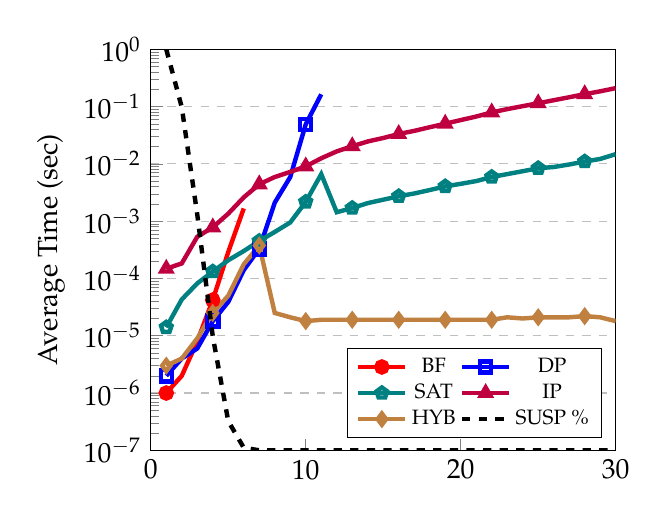
\begin{tikzpicture}
    \begin{axis}[
        scale=.7,
        %title={Average checking time versus puzzle height for 10000 random width 8 puzzles},
        %xlabel={Puzzle Height},
        ylabel={Average Time (sec)},
        %width=3.4in,
        %height=2.5in,
        xmin=0, xmax=30,
        ytick pos=left,
        xtick pos=left,
        ymin=1e-7, ymax=1,
        legend pos=south east,
        legend style={legend columns=2, nodes={scale=0.75, transform shape}},
        ymajorgrids=true,
        grid style=dashed,
        ymode=log,
        cycle list name=color list,
        scale only axis,
        every axis plot/.append style={ultra thick},
      ]
      \addplot[mark=*, mark repeat=3, red]
      coordinates {
(1,0.000001)
(2,0.000002)
(3,0.000008)
(4,0.000042)
(5,0.000290)
(6,0.001668)
      };
      
      
      \addplot[mark=square, mark repeat=3, blue]
      coordinates {
(1,0.000002)
(2,0.000004)
(3,0.000006)
(4,0.000018)
(5,0.000039)
(6,0.000140)
(7,0.000330)
(8,0.002107)
(9,0.005892)
(10,0.049053)
(11,0.163843)
      };
      
      \addplot[mark=pentagon, mark repeat=3, teal]
      coordinates {
(1,0.000014)
(2,0.000043)
(3,0.000082)
(4,0.000132)
(5,0.000208)
(6,0.000301)
(7,0.000451)
(8,0.000649)
(9,0.000950)
(10,0.002174)
(11,0.006619)
(12,0.001433)
(13,0.001696)
(14,0.002068)
(15,0.002371)
(16,0.002722)
(17,0.003043)
(18,0.003496)
(19,0.004051)
(20,0.004487)
(21,0.005012)
(22,0.005906)
(23,0.006633)
(24,0.007448)
(25,0.008406)
(26,0.008819)
(27,0.009764)
(28,0.010991)
(29,0.012199)
(30,0.014788)
      };
      
      \addplot[mark=triangle, mark repeat=3, purple]
      coordinates {
(1,0.000148)
(2,0.000183)
(3,0.000535)
(4,0.000780)
(5,0.001353)
(6,0.002607)
(7,0.004405)
(8,0.005905)
(9,0.007247)
(10,0.009047)
(11,0.012536)
(12,0.016524)
(13,0.020360)
(14,0.024634)
(15,0.028322)
(16,0.033261)
(17,0.037690)
(18,0.043702)
(19,0.050287)
(20,0.058206)
(21,0.067089)
(22,0.079269)
(23,0.090435)
(24,0.101884)
(25,0.114451)
(26,0.129260)
(27,0.145687)
(28,0.164847)
(29,0.184864)
(30,0.210087)
      };

      \addplot[mark=diamond, mark repeat=3, brown]
      coordinates {
(1,0.000003)
(2,0.000004)
(3,0.000009)
(4,0.000025)
(5,0.000050)
(6,0.000177)
(7,0.000376)
(8,0.000025)
(9,0.000021)
(10,0.000018)
(11,0.000019)
(12,0.000019)
(13,0.000019)
(14,0.000019)
(15,0.000019)
(16,0.000019)
(17,0.000019)
(18,0.000019)
(19,0.000019)
(20,0.000019)
(21,0.000019)
(22,0.000019)
(23,0.000021)
(24,0.000020)
(25,0.000021)
(26,0.000021)
(27,0.000021)
(28,0.000022)
(29,0.000021)
(30,0.000018)
      };
      \addplot[style=dashed, black]
      coordinates{
        (0,0)
        (0,1)
      };
      \legend{BF, DP, SAT, IP, HYB, SUSP \%}
    \end{axis}
    \begin{axis}[
        scale only axis,
        scale=.7,
        %width=3.4in,
        %height=2.5in,
        %axis y line*=right,
        axis y line=none,
        ymin=0,ymax=100,
        xmin=0,xmax=30,
        axis x line=none,
        every axis plot/.append style={ultra thick},
        %ylabel={Percent SUSP},
        axis x line=none,
        ylabel style = {align=center},ylabel near ticks
        ]
      \addplot[style=dashed]
      coordinates {
(1,100.0)
(2,85.56)
(3,58.8)
(4,28.410000000000004)
(5,7.2700000000000005)
(6,0.65)
(7,0.0)
(8,0.0)
(9,0.0)
(10,0.0)
(11,0.0)
(12,0.0)
(13,0.0)
(14,0.0)
(15,0.0)
(16,0.0)
(17,0.0)
(18,0.0)
(19,0.0)
(20,0.0)
(21,0.0)
(22,0.0)
(23,0.0)
(24,0.0)
(25,0.0)
(26,0.0)
(27,0.0)
(28,0.0)
(29,0.0)
(30,0.0)
      }; \label{percentSUSP}
      %\legend{SUSP \%}
    \end{axis}
  \end{tikzpicture}

  \end{subfigure}%
  ~~~~~~~~~~~~~~~~~~~~~~~~~~~~~~~~~~
  \begin{subfigure}[t]{0.3\textwidth}
      \caption{Width 6 strong USP.}
  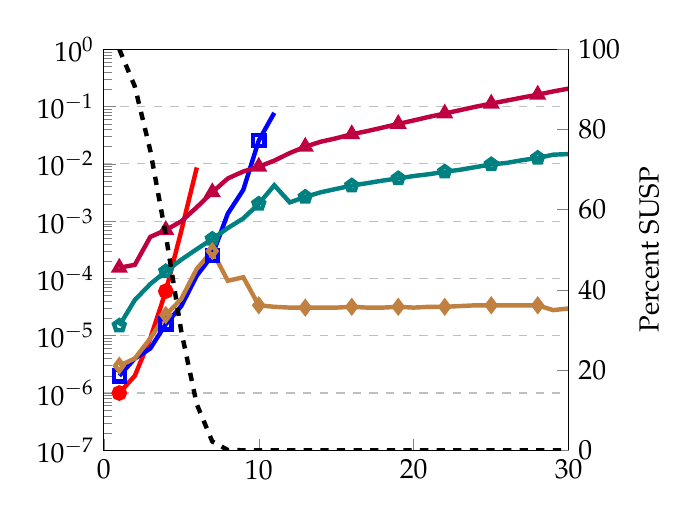
\begin{tikzpicture}
    \begin{axis}[
        scale=.7,
        %title={Average checking time versus puzzle height for 10000 random width 8 puzzles},
        %xlabel={Puzzle Height},
        %ylabel={Average Time (sec)},
        %width=3.4in,
        %height=2.5in,
        xmin=0, xmax=30,
        ytick pos=left,
        xtick pos=left,
        ymin=1e-7, ymax=1,
        legend pos=south east,
        legend style={legend columns=2},
        ymajorgrids=true,
        grid style=dashed,
        ymode=log,
        cycle list name=color list,
        scale only axis,
        every axis plot/.append style={ultra thick},
      ]
      
      \addplot[mark=*, mark repeat=3, red]
      coordinates {
(1,0.000001)
(2,0.000002)
(3,0.000009)
(4,0.000060)
(5,0.000679)
(6,0.008650)
      };
      
      
      \addplot[mark=square, mark repeat=3, blue]
      coordinates {
(1,0.000002)
(2,0.000004)
(3,0.000006)
(4,0.000016)
(5,0.000033)
(6,0.000112)
(7,0.000253)
(8,0.001355)
(9,0.003520)
(10,0.025636)
(11,0.077827)
      };
      
      \addplot[mark=pentagon, mark repeat=3, teal]
      coordinates {
(1,0.000015)
(2,0.000042)
(3,0.000080)
(4,0.000133)
(5,0.000213)
(6,0.000325)
(7,0.000489)
(8,0.000758)
(9,0.001117)
(10,0.002009)
(11,0.004235)
(12,0.002129)
(13,0.002650)
(14,0.003195)
(15,0.003661)
(16,0.004184)
(17,0.004614)
(18,0.005113)
(19,0.005574)
(20,0.006143)
(21,0.006614)
(22,0.007291)
(23,0.007908)
(24,0.008801)
(25,0.009797)
(26,0.010409)
(27,0.011608)
(28,0.012684)
(29,0.014477)
(30,0.014838)
      };
      
      \addplot[mark=triangle, mark repeat=3, purple]
      coordinates {
(1,0.000154)
(2,0.000173)
(3,0.000532)
(4,0.000701)
(5,0.000994)
(6,0.001749)
(7,0.003201)
(8,0.005568)
(9,0.007367)
(10,0.008928)
(11,0.011399)
(12,0.015474)
(13,0.019977)
(14,0.024378)
(15,0.028027)
(16,0.032904)
(17,0.037362)
(18,0.043104)
(19,0.049805)
(20,0.057387)
(21,0.066355)
(22,0.075801)
(23,0.086858)
(24,0.099631)
(25,0.112705)
(26,0.127511)
(27,0.143807)
(28,0.161481)
(29,0.184042)
(30,0.206666)
      };

      \addplot[mark=diamond, mark repeat=3, brown]
      coordinates {
(1,0.000003)
(2,0.000004)
(3,0.000009)
(4,0.000023)
(5,0.000044)
(6,0.000148)
(7,0.000301)
(8,0.000091)
(9,0.000105)
(10,0.000034)
(11,0.000032)
(12,0.000031)
(13,0.000031)
(14,0.000031)
(15,0.000031)
(16,0.000032)
(17,0.000031)
(18,0.000031)
(19,0.000032)
(20,0.000031)
(21,0.000032)
(22,0.000032)
(23,0.000033)
(24,0.000034)
(25,0.000034)
(26,0.000034)
(27,0.000034)
(28,0.000034)
(29,0.000028)
(30,0.000030)
      };
      %\legend{BF, DP, SAT, IP, Hybrid}
    \end{axis}
    \begin{axis}[
        scale only axis,
        scale=.7,
        %width=3.4in,
        %height=2.5in,
        axis y line*=right,
        ymin=0,ymax=100,
        xmin=0,xmax=30,
        axis x line=none,
        every axis plot/.append style={ultra thick},
        ylabel={Percent SUSP},
        axis x line=none,
        ylabel style = {align=center},ylabel near ticks
        ]
      \addplot[style=dashed]
      coordinates {
        (1,100.0)
(2,90.75999999999999)
(3,74.72999999999999)
(4,53.690000000000005)
(5,29.65)
(6,11.48)
(7,2.19)
(8,0.08)
(9,0.01)
(10,0.0)
(11,0.0)
(12,0.0)
(13,0.0)
(14,0.0)
(15,0.0)
(16,0.0)
(17,0.0)
(18,0.0)
(19,0.0)
(20,0.0)
(21,0.0)
(22,0.0)
(23,0.0)
(24,0.0)
(25,0.0)
(26,0.0)
(27,0.0)
(28,0.0)
(29,0.0)
(30,0.0)
      }; \label{percentSUSP}
      %\legend{SUSP \%}
    \end{axis}
  \end{tikzpicture}

  \end{subfigure}

  \begin{subfigure}[t]{0.3\textwidth}
    \vspace{1.5ex}
    \caption{Width 7 strong USP.}
  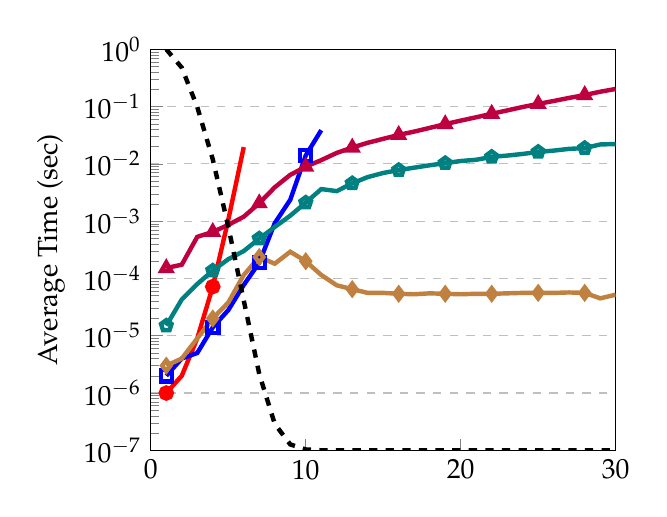
\begin{tikzpicture}
    \begin{axis}[
        scale=.7,
        %title={Average checking time versus puzzle height for 10000 random width 8 puzzles},
        %xlabel={Puzzle Height},
        ylabel={Average Time (sec)},
        %width=3.4in,
        %height=2.5in,
        xmin=0, xmax=30,
        ytick pos=left,
        xtick pos=left,
        ymin=1e-7, ymax=1,
        legend pos=south east,
        legend style={legend columns=2},
        ymajorgrids=true,
        grid style=dashed,
        ymode=log,
        cycle list name=color list,
        scale only axis,
        every axis plot/.append style={ultra thick},
      ]
      
      \addplot[mark=*, mark repeat=3, red]
      coordinates {
(1,0.000001)
(2,0.000002)
(3,0.000009)
(4,0.000072)
(5,0.001053)
(6,0.019641)
      };
      
      
      \addplot[mark=square, mark repeat=3, blue]
      coordinates {
        (1,0.000002)
(2,0.000004)
(3,0.000005)
(4,0.000014)
(5,0.000028)
(6,0.000077)
(7,0.000189)
(8,0.000923)
(9,0.002358)
(10,0.014033)
(11,0.038762)
      };
      
      \addplot[mark=pentagon, mark repeat=3, teal]
      coordinates {
(1,0.000015)
(2,0.000043)
(3,0.000080)
(4,0.000137)
(5,0.000217)
(6,0.000301)
(7,0.000497)
(8,0.000792)
(9,0.001247)
(10,0.002107)
(11,0.003634)
(12,0.003348)
(13,0.004578)
(14,0.005887)
(15,0.006944)
(16,0.007799)
(17,0.008594)
(18,0.009459)
(19,0.010304)
(20,0.011223)
(21,0.011809)
(22,0.013254)
(23,0.013968)
(24,0.014924)
(25,0.016176)
(26,0.017060)
(27,0.018297)
(28,0.018889)
(29,0.021833)
(30,0.022220)
      };
      
      \addplot[mark=triangle, mark repeat=3, purple]
      coordinates {
(1,0.000152)
(2,0.000174)
(3,0.000533)
(4,0.000649)
(5,0.000861)
(6,0.001198)
(7,0.002055)
(8,0.003904)
(9,0.006433)
(10,0.008940)
(11,0.011625)
(12,0.015559)
(13,0.019298)
(14,0.023393)
(15,0.027376)
(16,0.032076)
(17,0.036646)
(18,0.042521)
(19,0.049422)
(20,0.056971)
(21,0.065176)
(22,0.074952)
(23,0.085829)
(24,0.098522)
(25,0.111465)
(26,0.125384)
(27,0.141956)
(28,0.159088)
(29,0.181931)
(30,0.203126)
      };

      \addplot[mark=diamond, mark repeat=3, brown]
      coordinates {
(1,0.000003)
(2,0.000004)
(3,0.000009)
(4,0.000020)
(5,0.000038)
(6,0.000115)
(7,0.000236)
(8,0.000181)
(9,0.000293)
(10,0.000200)
(11,0.000115)
(12,0.000076)
(13,0.000065)
(14,0.000056)
(15,0.000056)
(16,0.000054)
(17,0.000053)
(18,0.000055)
(19,0.000054)
(20,0.000053)
(21,0.000054)
(22,0.000054)
(23,0.000055)
(24,0.000056)
(25,0.000056)
(26,0.000056)
(27,0.000057)
(28,0.000056)
(29,0.000045)
(30,0.000052)
      };
      \addplot[style=dashed, black]
      coordinates{
        (0,0)
        (0,1)
      };
      %\legend{BF, DP, SAT, IP, Hybrid, SUSP \%}
    \end{axis}
    \begin{axis}[
        scale only axis,
        scale=.7,
        %width=3.4in,
        %height=2.5in,
        %axis y line*=right,
        axis y line=none,
        ymin=0,ymax=100,
        xmin=0,xmax=30,
        axis x line=none,
        every axis plot/.append style={ultra thick},
        %ylabel={Percent SUSP},
        axis x line=none,
        ylabel style = {align=center},ylabel near ticks
        ]
      \addplot[style=dashed]
      coordinates {
(1,100.0)
(2,95.44)
(3,85.61999999999999)
(4,72.59)
(5,55.82)
(6,37.38)
(7,19.040000000000003)
(8,6.59)
(9,1.47)
(10,0.22)
(11,0.01)
(12,0.0)
(13,0.0)
(14,0.0)
(15,0.0)
(16,0.0)
(17,0.0)
(18,0.0)
(19,0.0)
(20,0.0)
(21,0.0)
(22,0.0)
(23,0.0)
(24,0.0)
(25,0.0)
(26,0.0)
(27,0.0)
(28,0.0)
(29,0.0)
(30,0.0)
      }; \label{percentSUSP}
      %\legend{SUSP \%}
    \end{axis}
  \end{tikzpicture}

  \end{subfigure}%
  ~~~~~~~~~~~~~~~~~~~~~~~~~~~~~~~~~~
  \begin{subfigure}[t]{0.3\textwidth}
    \vspace{1.5ex}
    \caption{Width 8 strong USP.}
  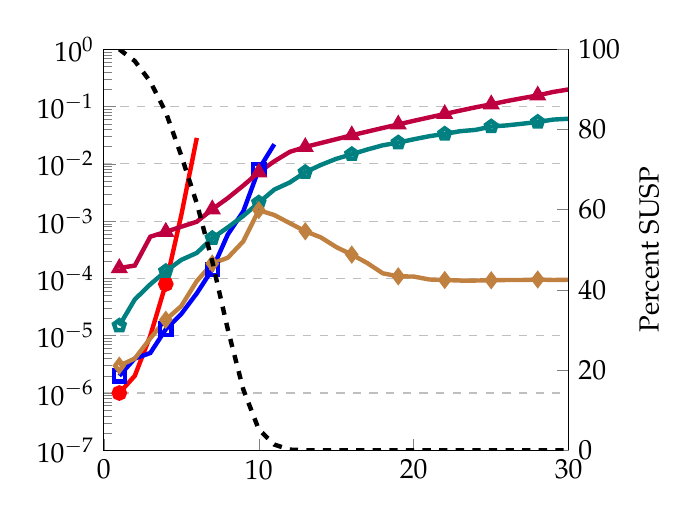
\begin{tikzpicture}
    \begin{axis}[
        scale=.7,
        %title={Average checking time versus puzzle height for 10000 random width 8 puzzles},
        %xlabel={Puzzle Height},
        %ylabel={Average Time (sec)},
        %width=3.4in,
        %height=2.5in,
        xmin=0, xmax=30,
        ytick pos=left,
        xtick pos=left,
        ymin=1e-7, ymax=1,
        legend pos=south east,
        legend style={legend columns=2},
        ymajorgrids=true,
        grid style=dashed,
        ymode=log,
        cycle list name=color list,
        scale only axis,
        every axis plot/.append style={ultra thick},
      ]
      
      \addplot[mark=*, mark repeat=3, red]
      coordinates {
(1,0.000001)
(2,0.000002)
(3,0.000010)
(4,0.000080)
(5,0.001278)
(6,0.028475)
      };
      
      
      \addplot[mark=square, mark repeat=3, blue]
      coordinates {
(1,0.000002)
(2,0.000004)
(3,0.000005)
(4,0.000013)
(5,0.000024)
(6,0.000055)
(7,0.000144)
(8,0.000586)
(9,0.001485)
(10,0.008024)
(11,0.022047)
      };
      
      \addplot[mark=pentagon, mark repeat=3, teal]
      coordinates {
(1,0.000015)
(2,0.000043)
(3,0.000079)
(4,0.000134)
(5,0.000211)
(6,0.000279)
(7,0.000505)
(8,0.000779)
(9,0.001235)
(10,0.002107)
(11,0.003558)
(12,0.004742)
(13,0.007168)
(14,0.009571)
(15,0.012269)
(16,0.014747)
(17,0.017819)
(18,0.021106)
(19,0.023533)
(20,0.026900)
(21,0.030405)
(22,0.033466)
(23,0.037229)
(24,0.039283)
(25,0.044903)
(26,0.046999)
(27,0.050242)
(28,0.053942)
(29,0.059373)
(30,0.061401)
      };
      
      \addplot[mark=triangle, mark repeat=3, purple]
      coordinates {
(1,0.000152)
(2,0.000168)
(3,0.000536)
(4,0.000653)
(5,0.000800)
(6,0.000978)
(7,0.001614)
(8,0.002529)
(9,0.004187)
(10,0.007130)
(11,0.011094)
(12,0.016223)
(13,0.019727)
(14,0.023134)
(15,0.026999)
(16,0.031622)
(17,0.036585)
(18,0.042355)
(19,0.048855)
(20,0.056438)
(21,0.064877)
(22,0.074264)
(23,0.085323)
(24,0.097307)
(25,0.109676)
(26,0.124883)
(27,0.140305)
(28,0.156828)
(29,0.180271)
(30,0.199624)
      };

      \addplot[mark=diamond, mark repeat=3, brown]
      coordinates {
(1,0.000003)
(2,0.000004)
(3,0.000009)
(4,0.000019)
(5,0.000033)
(6,0.000090)
(7,0.000182)
(8,0.000230)
(9,0.000444)
(10,0.001559)
(11,0.001280)
(12,0.000924)
(13,0.000666)
(14,0.000522)
(15,0.000353)
(16,0.000261)
(17,0.000186)
(18,0.000123)
(19,0.000109)
(20,0.000108)
(21,0.000096)
(22,0.000094)
(23,0.000092)
(24,0.000092)
(25,0.000093)
(26,0.000094)
(27,0.000094)
(28,0.000096)
(29,0.000094)
(30,0.000095)
      };
      %\legend{BF, DP, SAT, IP, Hybrid}
    \end{axis}
    \begin{axis}[
        scale only axis,
        scale=.7,
        %width=3.4in,
        %height=2.5in,
        axis y line*=right,
        ymin=0,ymax=100,
        xmin=0,xmax=30,
        axis x line=none,
        every axis plot/.append style={ultra thick},
        ylabel={Percent SUSP},
        axis x line=none,
        ylabel style = {align=center},ylabel near ticks
        ]
      \addplot[style=dashed]
      coordinates {
(1,100.0)
(2,97.08)
(3,91.94)
(4,84.31)
(5,73.49)
(6,61.59)
(7,47.099999999999994)
(8,30.18)
(9,15.18)
(10,5.21)
(11,1.44)
(12,0.16999999999999998)
(13,0.02)
(14,0.0)
(15,0.0)
(16,0.0)
(17,0.0)
(18,0.0)
(19,0.0)
(20,0.0)
(21,0.0)
(22,0.0)
(23,0.0)
(24,0.0)
(25,0.0)
(26,0.0)
(27,0.0)
(28,0.0)
(29,0.0)
(30,0.0)
      }; \label{percentSUSP}
      %\legend{SUSP \%}
    \end{axis}
  \end{tikzpicture}
  \end{subfigure}



  \begin{subfigure}[t]{0.3\textwidth}
    \vspace{1.5ex}
    \caption{Width 9 strong USP.}
  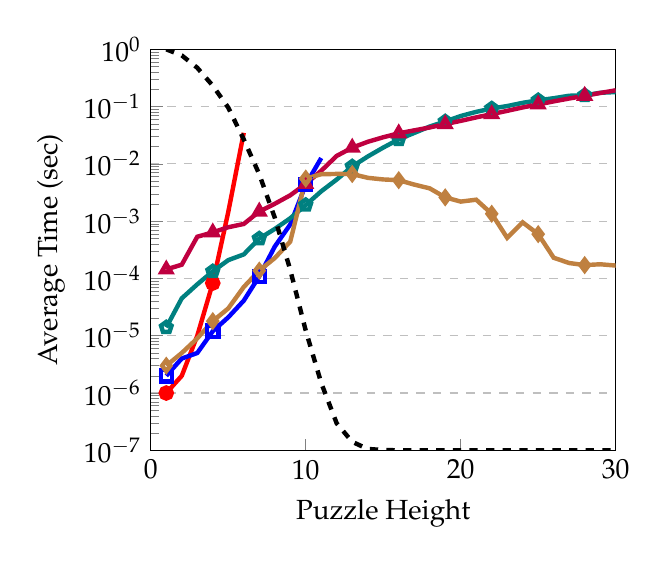
\begin{tikzpicture}
    \begin{axis}[
        scale=.7,
        %title={Average checking time versus puzzle height for 10000 random width 8 puzzles},
        xlabel={Puzzle Height},
        ylabel={Average Time (sec)},
        %width=3.4in,
        %height=2.5in,
        xmin=0, xmax=30,
        ytick pos=left,
        xtick pos=left,
        ymin=1e-7, ymax=1,
        legend pos=south east,
        legend style={legend columns=2},
        ymajorgrids=true,
        grid style=dashed,
        ymode=log,
        cycle list name=color list,
        scale only axis,
        every axis plot/.append style={ultra thick},
      ]
      
      \addplot[mark=*, mark repeat=3, red]
      coordinates {
(1,0.000001)
(2,0.000002)
(3,0.000010)
(4,0.000083)
(5,0.001447)
(6,0.034856)
      };
      
      
      \addplot[mark=square, mark repeat=3, blue]
      coordinates {
(1,0.000002)
(2,0.000004)
(3,0.000005)
(4,0.000012)
(5,0.000021)
(6,0.000041)
(7,0.000109)
(8,0.000360)
(9,0.000876)
(10,0.004350)
(11,0.012662)
      };
      
      \addplot[mark=pentagon, mark repeat=3, teal]
      coordinates {
(1,0.000014)
(2,0.000045)
(3,0.000079)
(4,0.000133)
(5,0.000209)
(6,0.000263)
(7,0.000497)
(8,0.000731)
(9,0.001125)
(10,0.001914)
(11,0.003326)
(12,0.005342)
(13,0.009016)
(14,0.013461)
(15,0.019261)
(16,0.026867)
(17,0.034681)
(18,0.044907)
(19,0.055021)
(20,0.068536)
(21,0.080987)
(22,0.092563)
(23,0.102250)
(24,0.116448)
(25,0.128873)
(26,0.140122)
(27,0.154784)
(28,0.157334)
(29,0.174383)
(30,0.179453)
      };
      
      \addplot[mark=triangle, mark repeat=3, purple]
      coordinates {
(1,0.000144)
(2,0.000174)
(3,0.000535)
(4,0.000637)
(5,0.000784)
(6,0.000894)
(7,0.001474)
(8,0.002012)
(9,0.002833)
(10,0.004460)
(11,0.007585)
(12,0.013803)
(13,0.019238)
(14,0.024299)
(15,0.029166)
(16,0.034196)
(17,0.038492)
(18,0.043241)
(19,0.049450)
(20,0.056393)
(21,0.064838)
(22,0.073858)
(23,0.084390)
(24,0.096774)
(25,0.109239)
(26,0.123410)
(27,0.138516)
(28,0.154470)
(29,0.172965)
(30,0.192481)
      };

      \addplot[mark=diamond, mark repeat=3, brown]
      coordinates {
(1,0.000003)
(2,0.000005)
(3,0.000009)
(4,0.000018)
(5,0.000030)
(6,0.000071)
(7,0.000137)
(8,0.000227)
(9,0.000440)
(10,0.005532)
(11,0.006604)
(12,0.006680)
(13,0.006660)
(14,0.005714)
(15,0.005352)
(16,0.005199)
(17,0.004353)
(18,0.003739)
(19,0.002604)
(20,0.002197)
(21,0.002372)
(22,0.001346)
(23,0.000511)
(24,0.000952)
(25,0.000594)
(26,0.000230)
(27,0.000186)
(28,0.000171)
(29,0.000177)
(30,0.000168)
      };
      \addplot[style=dashed, black]
      coordinates{
        (0,0)
        (0,1)
      };
      %\legend{BF, DP, SAT, IP, Hybrid, SUSP \%}
    \end{axis}
    \begin{axis}[
        scale only axis,
        scale=.7,
        %width=3.4in,
        %height=2.5in,
        %axis y line*=right,
        axis y line=none,
        ymin=0,ymax=100,
        xmin=0,xmax=30,
        axis x line=none,
        every axis plot/.append style={ultra thick},
        %ylabel={Percent SUSP},
        axis x line=none,
        ylabel style = {align=center},ylabel near ticks
        ]
      \addplot[style=dashed]
      coordinates {
(1,100.0)
(2,98.48)
(3,95.39999999999999)
(4,90.94)
(5,85.47)
(6,77.53)
(7,68.85)
(8,58.040000000000006)
(9,45.01)
(10,29.86)
(11,16.78)
(12,6.710000000000001)
(13,2.11)
(14,0.33999999999999997)
(15,0.06999999999999999)
(16,0.0)
(17,0.0)
(18,0.0)
(19,0.0)
(20,0.0)
(21,0.0)
(22,0.0)
(23,0.0)
(24,0.0)
(25,0.0)
(26,0.0)
(27,0.0)
(28,0.0)
(29,0.0)
(30,0.0)
      }; \label{percentSUSP}
      %\legend{SUSP \%}
    \end{axis}
  \end{tikzpicture}

  \end{subfigure}%
  ~~~~~~~~~~~~~~~~~~~~~~~~~~~~~~~~~~
  \begin{subfigure}[t]{0.3\textwidth}
    \vspace{1.5ex}
    \caption{Width 10 strong USP.}
  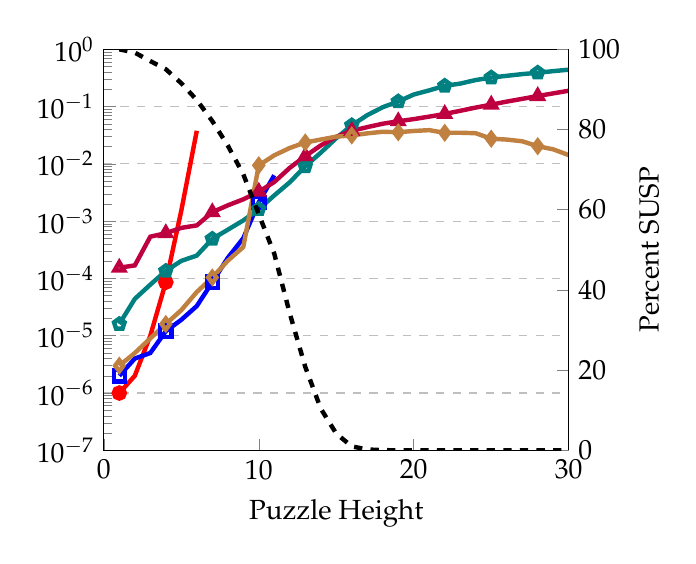
\begin{tikzpicture}
    \begin{axis}[
        scale=.7,
        %title={Average checking time versus puzzle height for 10000 random width 8 puzzles},
        xlabel={Puzzle Height},
        %ylabel={Average Time (sec)},
        %width=3.4in,
        %height=2.5in,
        xmin=0, xmax=30,
        ytick pos=left,
        xtick pos=left,
        ymin=1e-7, ymax=1,
        legend pos=south east,
        legend style={legend columns=2},
        ymajorgrids=true,
        grid style=dashed,
        ymode=log,
        cycle list name=color list,
        scale only axis,
        every axis plot/.append style={ultra thick},
      ]
      
      \addplot[mark=*, mark repeat=3, red]
      coordinates {
(1,0.000001)
(2,0.000002)
(3,0.000010)
(4,0.000086)
(5,0.001527)
(6,0.037871)
      };
      
      
      \addplot[mark=square, mark repeat=3, blue]
      coordinates {
(1,0.000002)
(2,0.000004)
(3,0.000005)
(4,0.000012)
(5,0.000019)
(6,0.000033)
(7,0.000086)
(8,0.000229)
(9,0.000504)
(10,0.002137)
(11,0.006329)
      };
      
      \addplot[mark=pentagon, mark repeat=3, teal]
      coordinates {
(1,0.000016)
(2,0.000044)
(3,0.000078)
(4,0.000135)
(5,0.000203)
(6,0.000251)
(7,0.000491)
(8,0.000709)
(9,0.001031)
(10,0.001623)
(11,0.002816)
(12,0.004783)
(13,0.009073)
(14,0.015697)
(15,0.028175)
(16,0.047146)
(17,0.070970)
(18,0.097643)
(19,0.122891)
(20,0.162530)
(21,0.192221)
(22,0.230472)
(23,0.252367)
(24,0.291011)
(25,0.321245)
(26,0.344867)
(27,0.369262)
(28,0.389873)
(29,0.416138)
(30,0.441104)
      };
      
      \addplot[mark=triangle, mark repeat=3, purple]
      coordinates {
(1,0.000154)
(2,0.000169)
(3,0.000536)
(4,0.000617)
(5,0.000764)
(6,0.000844)
(7,0.001435)
(8,0.001891)
(9,0.002407)
(10,0.003265)
(11,0.004831)
(12,0.008536)
(13,0.013664)
(14,0.021003)
(15,0.029735)
(16,0.037749)
(17,0.043829)
(18,0.050243)
(19,0.055525)
(20,0.060482)
(21,0.066943)
(22,0.074377)
(23,0.084496)
(24,0.096253)
(25,0.108099)
(26,0.122322)
(27,0.136572)
(28,0.153064)
(29,0.170231)
(30,0.189359)
      };

      \addplot[mark=diamond, mark repeat=3, brown]
      coordinates {
(1,0.000003)
(2,0.000005)
(3,0.000009)
(4,0.000016)
(5,0.000028)
(6,0.000058)
(7,0.000104)
(8,0.000204)
(9,0.000354)
(10,0.009436)
(11,0.014118)
(12,0.018966)
(13,0.023669)
(14,0.026621)
(15,0.029888)
(16,0.031436)
(17,0.034132)
(18,0.036392)
(19,0.035710)
(20,0.037570)
(21,0.038830)
(22,0.034886)
(23,0.035004)
(24,0.034309)
(25,0.027510)
(26,0.026576)
(27,0.024817)
(28,0.020389)
(29,0.017953)
(30,0.014241)
      };
      %\legend{BF, DP, SAT, IP, Hybrid}
    \end{axis}
    \begin{axis}[
        scale only axis,
        scale=.7,
        %width=3.4in,
        %height=2.5in,
        axis y line*=right,
        ymin=0,ymax=100,
        xmin=0,xmax=30,
        axis x line=none,
        every axis plot/.append style={ultra thick},
        ylabel={Percent SUSP},
        axis x line=none,
        ylabel style = {align=center},ylabel near ticks
        ]
      \addplot[style=dashed]
      coordinates {
(1,100.0)
(2,99.18)
(3,97.07000000000001)
(4,95.04)
(5,91.55)
(6,87.35000000000001)
(7,82.11)
(8,76.0)
(9,68.86)
(10,58.87)
(11,49.02)
(12,34.14)
(13,20.8)
(14,10.4)
(15,4.17)
(16,0.98)
(17,0.21)
(18,0.04)
(19,0.0)
(20,0.0)
(21,0.0)
(22,0.0)
(23,0.0)
(24,0.0)
(25,0.0)
(26,0.0)
(27,0.0)
(28,0.0)
(29,0.0)
(30,0.0)
      }; \label{percentSUSP}
      %\legend{SUSP \%}
    \end{axis}
  \end{tikzpicture}
  \end{subfigure}

  \vspace{-2ex}
  \caption{Log plots of the average running times for 10000 random puzzles of widths
    five to ten. Note that the legend in (a) applies to all six plots,
    and that the axes are named only the edge of the page.  Each plot
    describes the behavior of five algorithms brute force (BF),
    dynamic programming (DP), reduction to satisfiability (SAT),
    reduction to integer programming (IP), and the hybrid algorithm
    (HYB).  The final dashed line indicates the percentage of SUSP
    found among the 10000 random puzzles.}
  \label{fig:perform}
\end{figure}
  


\section{Conclusions}
\label{sec:conclusion}

We initiated the first study of the verification strong USP and
developed practical software for both verifying and searching for
them.  We give tight results on the maximum size of width-$k$
strong USP for $k \le 5$.  Although our results do not produce a new
upper bound on the running time of matrix multiplication, they
demonstrate there is promise in this approach. %the uniquely solvable puzzle approach.
There are a number of open questions.
%The immediate open question is:
What are tight bounds on maximum size
strong USP for $k \ge 6$ and do these bound lead to asymptotically
faster algorithms for matrix multiplication?
Is strong USP verification \NP-complete?
The main bottleneck in
our work is the size of the search space:
%This leads to a number of open questions:
Can the size of the search space be lowered by modding out by symmetries of puzzles?  Preliminary work
suggests this is possible, but not yet sufficient to exhaustively
search width-6 strong USP.
%% Is there a way to identify rows
%% that can be added to a strong USP other than examining all possible
%% rows and checking whether the puzzle remains a strong USP?
%% Are there
%% other search strategies that would be more effective on this search
%% space?  

\section{Acknowledgments}

The second and third authors would like to the Union College
Summer Research Fellowship for supporting their work.

\bibliographystyle{customurlbst/alphaurlpp} \bibliography{references}

\appendix

\section{Bidirectional Search}

\label{app:bi}

\autoref{alg:bi} describes a recursive
bidirectional strong USP verification algorithm that using the 3D
matching instance.

\begin{algorithm}[h]
  \caption{: Bidirectional}
  \label{alg:bi}
\begin{algorithmic}[1]
  \Require{An $(s,k)$-puzzle $P$.}
  \Ensure{YES, if $P$ is a strong USP and NO otherwise.}
  \Function{VerifyBidirectional}{$P$}
  \State{Let $T = \emptyset$.}
  \State{Construct 3DM instance $H_P$.}
  \Function{SearchHalf}{$\ell, Q,\ell_Q, R,\ell_R, \delta, t$}
  \If{$\ell = t$}
    \If{$\delta = 1$} \Comment{Forward Base Case}
      \State{Insert $(Q,R)$ into $T$.}
      \State{\Return{$false$}.}
    \Else \Comment{Reverse Base Case}
      \If{$(P-Q, P-R) \in T$} \State{\Return{$true$}.} \Else \State{\Return{$false$}.} \EndIf
    \EndIf
  \EndIf
  \State{$result = false$.} \Comment{Recursive Case}
  \For{$\ell'_Q = \ell_Q + 1$ to $s$}
    \For{$\ell'_R = \ell_R + 1$ to $s$}
      \If{$(p_\ell, p_{\ell'_Q}, p_{\ell'_R}) \in H_P$}
        \State{$result = result~\vee$ \textsc{SearchHalf}$(\ell + \delta, Q \cup \set{p_{\ell'_Q}}, \ell'_Q, R \cup \set{p_{\ell'_R}}, \ell'_R, \delta, t)$.}
      \EndIf
    \EndFor
  \EndFor
  \State{\Return{$result$.}}
  \EndFunction

  \State{\textsc{SearchHalf}$(1,\emptyset, 0, \emptyset, 0, 1, \lfloor s / 2 \rfloor + 1)$.}
  \State{\Return{\textsc{SearchHalf}$(s, \emptyset, 0, \emptyset, 0, -1, \lfloor s/2 \rfloor)$}.}
  \EndFunction
\end{algorithmic}
\end{algorithm}

\autoref{alg:bi} consists of two phases. Let $t = \lfloor s/2
\rfloor$. The first phase determines all possible sets $Q,R \sse P$
with $|Q| = |R| = t$ such that there is 3D matching $M_1$ of $H_P$
when restricted to the vertices $\set{p_1,p_2, \ldots, p_t} \sqcup Q
\sqcup R$.  The sets $Q,R$ satisfying the requirement are stored in a
table $T$ during the first phase on Line 6.  The second phase
determines all possible sets $Q,R \sse P$ with $|Q| = |R| = s - t$
such that there is a 3D matching $M_2$ of $H_P$ when restricted to the
vertices $\set{p_{t+1},p_{t+2},\ldots,p_s} \sqcup Q \sqcup R$.  For
each pair $(Q,R)$ the algorithm determines in the second phase it
checks whether $(P - Q, P - R)$ was inserted into $T$ during the first
phase.  If the pair is present it means that there is a 3D matching of
$H_P$ which is $M = M_1 \cup M_2$.  This works because $M_1$ and $M_2$
are partial 3D matchings and vertex disjoint.  This is because $M_1$
is a 3D matching on $\set{p_1,\ldots,p_t}$ and $M_2$ is a 3D matching
on $\set{p_{t+1},\ldots p_s}$, and because in Line 9 of
\autoref{alg:bi} the lookup is performed on the complementary sets.
The second phase returns whether a complete matching could be found,
and hence by \autoref{lem:verify-to-3dm} whether $P$ is a strong USP.
(Note that the first phase always returns $false$.)

The running time of this algorithm is dominated by the number of pairs
of sets $(Q,R)$ it examines.  Observe that rows of $P$ are considered
in order in Lines 14 \& 15.  Further, the algorithm tracks the index
of last elements added to $Q$ and $R$ in $\ell_Q$ and $\ell_R$
respectively.  The algorithm only adds new elements to $Q$ or $R$ that
have higher indexes than ones previously added.  Altogether this
implies that each pair of sets $(Q,R)$ is only considered at most once
during a phase.  Since $Q, R \sse P$, there are at most $2^s \cdot
2^s$ pairs $(Q,R)$.  This means that \textsc{SearchHalf} is called at
most $4^s$ times during each phase.  Hence the running time of the
algorithm is $O(4^s \cdot s^2 \cdot \poly(s) + T_{3DM}(s,k))$ where
$s^2$ factor comes from the inner loops and $T_{3DM}(s,k)$ accounts
for the time to construct $H_P$.  The memory requirements of
\autoref{alg:bi} are similarly high -- the first phase uses $O(4^s
\cdot s)$ to store $T$.

Note that \autoref{alg:bi} does not early terminate on $P$ that are
strong USP, because it must search through all pairs before
determining that none can be found.  The algorithm could be modified
to allow early termination when $P$ is not a strong USP by causing the
second phase of search to immediately return in Line 17 once the first
3D matching witness has been located.  However, this still requires
the first phase to run to completion.  A remedy for this would be to
run both phases in parallel and have them check against each other.
This would substantially complicate the implementation, and not
substantially improve the practical running time for puzzles that are
strong USP.

In the implementation of \autoref{alg:bi} we represented the sets
$Q,R$ using bit sets encoded into a single 64-bit long.  This
permitted it to represent these sets for $s \le 32$.  We implemented
$T$ using a hash table (\texttt{map}s from the C++ standard template
library).  These choices made the basic data structure operations in
implementation effectively constant time, and have low memory overhead
beyond the contents of $T$.

Note that more advanced techniques like those of Bj\"{o}rklund et
al.~can acheive a better asymptotic time of $O(2^s\poly(s))$
\cite{bhkk17}.  We chose not to implement their algorithm, because we
judged that it would not substantially increase the domain of which
verification was possible.  

\section{Reduction to SAT}

\label{app:sat}

\begin{algorithm}[h]
  \caption{: Reduction to satisfiability}
  \label{alg:sat}
\begin{algorithmic}[1]
  \Require{An $(s,k)$-puzzle $P$.}
  \Ensure{YES, if $P$ is a strong USP and NO otherwise.}
  \Function{VerifySAT}{$P$}
  \State{Construct 3DM instance $H_P$.}
  \State{Construct CNF formula $\Psi_P$.}
  \If{$\Psi_P$ is satisfiable}
  \State{\Return NO}
  \Else
  \State{\Return YES}
  \EndIf
  \EndFunction
\end{algorithmic}
\end{algorithm}


\section{Reduction to IP}

\label{app:IP}


\begin{algorithm}[h]
  \caption{: Reduction to mixed integer programming}
  \label{alg:mip}
\begin{algorithmic}[1]
  \Require{An $(s,k)$-puzzle $P$.}
  \Ensure{YES, if $P$ is a strong USP and NO otherwise.}
  \Function{VerifyIP}{$P$}
  \State{Construct 3DM instance $H_P$.}
  \State{Create empty integer program $Q$ with Boolean variables $\condset{M_{u,v,w}}{u,v,w \in P}$.}
  \State{Add constraints of \autoref{eqn:cons1}, \autoref{eqn:cons2}, and \autoref{eqn:cons3} to $Q$.}
  \If{\textsc{IsFeasible}$(Q)$}
  \State{\Return{NO}.}
  \Else
  \State{\Return{YES}.}
  \EndIf
  \EndFunction
\end{algorithmic}
\end{algorithm}

\section{Greedy Heuristic}

\label{app:greedy}

\begin{algorithm}[h]
  \caption{: (Random) Greedy Heuristic}
  \label{alg:random-greedy}
\begin{algorithmic}[1]
  \Require{An $(s,k)$-puzzle $P$, and iteration bound $t$.}
  \Ensure{NO, if a witness is found for $P$ not being a strong USP, and MAYBE otherwise.}
  \Function{HeuristicGreedy}{$P$}
  \State{Construct 3DM instance $H_P$.}
  \For{$i = 1$ to $t$}
    \For{$u \in P$}
      \State{$cts[u] = \sum_{v,w \in P} H_P(u,v,w)$.} \Comment{Number of edges incident vertex $u$.}
    \EndFor
    \State{Let $U,V,W = \emptyset.$}
    \State{Let $m = 0.$} \Comment{Number of hyperedges in matching.}
    \While{$m < s$} 
      \State{Select $u \in \condset{u \in \bar{U}}{cts[u] = \max_{v \in \bar{U}} cts[v]}$ uniformly at random.}
      \If{$cts[u] = 0$} break. \EndIf
      \State{Select $(v,w) \in \condset{(v,w) \in \bar{V} \times \bar{W}}{H_P(u,v,w) = 1}$ uniformly at random.}
      \For{$v' \in P$} \Comment{Update edge counts.}
        \For{$w' \in P$}
          \If{$(v',w') \in \bar{V} \times \bar{W}$ and $H_P(u,v',w') = 1$} $cts[u]\texttt{--}$. \EndIf
          \If{$(v',w') \in \bar{U} \times \bar{W}$ and $H_P(v',v,w') = 1$ and $v' \neq u$} $cts[v']\texttt{--}$. \EndIf
          \If{$(v',w') \in \bar{U} \times \bar{V}$ and $H_P(v',w',w) = 1$ and $v' \neq u$ and $v' \neq v$} $cts[v']\texttt{--}$. \EndIf
        \EndFor
      \EndFor
      \State{$U = U \cup \set{u}$.} \Comment{Add edge to matching.}
      \State{$V = V \cup \set{v}$.}
      \State{$W = W \cup \set{w}$.}
      \State{$m = m + 1.$}
      \EndWhile
    \If {$m > s$} \Return{NO}. \Comment{3DM found so not SUSP, halt.} \EndIf
  \EndFor
  \State{\Return{MAYBE}.}
  \EndFunction
\end{algorithmic}
\end{algorithm}

The array $cts$ is used to store the number of edges $cts[u]$ that
remain associated with vertex $u$ along the first coordinate.  Much of
the algorithm is devoted to maintaining this invariant.  The sets
$U,V,W$ store the vertices along the three coordinates, respectively,
that have already been incorporated into the partial 3D matching.
Like in \autoref{alg:bi} we do not store the matching itself, only the
vertices involved.  The break at Line 10 triggers when the partial 3D
matching is a dead end and cannot be extended into a full 3D matching.
The condition of Line 21 is true when a full 3D matching has been
constructed and causes the algorithm to return that $P$ is not a
strong USP.

The running time of this algorithm is $O(s^3 t + T_{3DM}(s,k))$, where
$T_{3DM}(s,k)$ is the time required to construct 3D matching instances
from $(s,k)$-puzzles.  This algorithm has the potential to be
considerably slower than the downward-closure heuristic, and in
practice we set $t = s^3$.  However, the main loop can terminate early
at Line 10 when it fails to extend the 3D matching this permits the
expected time to much less than the worst case.  For a puzzle $P$ that
is a strong USP, the heuristic takes the full $\Omega(s^3 t +
T_{3DM}(s,k))$ time.





\section{2D Matching Heuristic}

\label{app:2dmatching}

The final heuristic we present is one-sided in the opposite direction
of the others, it may return YES or MAYBE.  In order for a hypergraph
$H_P$ to have a 3D matching it must be the case that when any one of
the three parts of vertices of $H_P$ is projected away the resulting
bipartite graph has a perfect matching.  Thus we can witness that
there is no 3D matching by determining that one of three projected
bipartite graphs $H_P|_1, H_P|_2, H_P|_3$ does not have a perfect
matching.

\begin{algorithm}[h]
  \caption{: 2D Matching Heuristic}
  \label{alg:2dm}
\begin{algorithmic}[1]
  \Require{An $(s,k)$-puzzle $P$.}
  \Ensure{YES, if $P$ is found to be strong USP, and MAYBE otherwise.}
  \Function{Heuristic2DMatching}{$P$}
  \State{Construct 3DM instance $H_P.$}
  \State{\texttt{// Construct projections.}}
  \State{Define projection $H_P|_1(b,c) = \vee_{a \in [s]} H_P(a,b,c)$.}
  \State{Define projection $H_P|_2(a,c) = \vee_{b \in [s]} H_P(a,b,c)$.}
  \State{Define projection $H_P|_3(a,b) = \vee_{c \in [s]} H_P(a,b,c)$.}

  \If{$H_P|_1, H_P|_2,$ and $H_P|_3$ have bipartite perfect matchings}
  \State{\Return{MAYBE.}}
  \Else
  \State{\Return{YES.}}
  \EndIf
  \EndFunction
\end{algorithmic}
\end{algorithm}

We can efficiently decide bipartite perfect matching using the
standard reduction to network flow and solve it using the
Ford-Faulkerson augmenting flow algorithm.  This approach yields an
algorithm that runs in time $O(s^3 + T_{3DM}(s,k))$, where
$T_{3DM}(s,k)$ is the time required to construct 3D matching instances
from $(s,k)$-puzzles.

In practice we found this heuristic not to be effective because the
projected $H_P|_i$ are typically dense graphs even if $H_P$ is not,
and so they are likely to have perfect matchings independently of
whether $H_P$ has a 3D matching.

\section{Generic Search}

\label{app:search}

\begin{algorithm}[h]
  \caption{: Depth-First Search}
  \label{alg:dfs}
\begin{algorithmic}[1]
  \Require{An integer $k \ge 0$, and a width-$k$ strong USP $P$.}
  \Ensure{The number $best$, which is the size of the largest strong USP that has $P$ as a subpuzzle.}

  \Function{DFS}{$k, P$}

  \State{Let $best = |P|$.}
  \State{Let $j$ be the index of the row $P_{|P|-1}$ in lexicographic order.}

  \For{$r = r_{j+1}$ to $r_{3^k-1}$}
    \State{Let $P' = P \cup \set{r}$.}
    \If{\Call{Verify}{$P'$}}
      \State{$best = \max(best, $ \Call{DFS}{$k, P'$}).}
    \EndIf
  \EndFor

  \State{\Return{$best$}.}

  \EndFunction
\end{algorithmic}
\end{algorithm}

\begin{algorithm}[h]
  \caption{: Breadth-First Search}
  \label{alg:bfs}
\begin{algorithmic}[1]
  \Require{An integer $k \ge 0$.}
  \Ensure{The number $best$, which is the size of the largest strong USP that has $P$ as a subpuzzle.}

  \Function{BFS}{$k$}

  \State{Let $Q$ be an empty queue.}
  \State{Push $\emptyset$ onto end of $Q$.}

  \While{$Q$ is not empty}
    \State{Pop head of $Q$ into $P$.}
    \State{Let $j$ be the index of the row $P_{|P|-1}$ in the lexicographic order of all rows.}
    \For{$r = r_{j+1}$ to $r_{3^k-1}$}
      \State{Let $P' = P \cup \set{r}$.}
      \If{\Call{Verify}{$P'$}}
        \State{Push $P'$ onto end of $Q$.}
        \State{$best = |P'|$.}
      \EndIf
    \EndFor
  \EndWhile

  \State{\Return{$best$}.}

  \EndFunction
\end{algorithmic}
\end{algorithm}



\end{document}
